%This template is designed by Zilu Rane and whole team of compilers
%So if your are using template so dont forget us
\documentclass[a4paper,12pt]{report}
\usepackage{geometry}
 \geometry{
 a4paper,
 left=30mm,
 top= 25mm,%%Actual value 15mm
 right=20mm,
 bottom=22mm,
 headheight=3mm,
 headsep=12mm
 }

\usepackage{graphicx}
\usepackage{titlesec,acronym,glossaries}
\usepackage{titleps}
\usepackage{indentfirst}
\usepackage{algorithmic}
\usepackage{ifthen}
\usepackage{multirow}
\usepackage{fancyhdr}
\usepackage{caption}
\usepackage{blindtext}
\usepackage{framed}
\usepackage{tocloft}
\usepackage{longtable}
\usepackage[utf8]{inputenc}
\usepackage[english]{babel}
\usepackage[nottoc]{tocbibind}
\usepackage{booktabs}
\usepackage{times}
%\usepackage{showframe}% check it to get margin lines
\usepackage{pdfpages}
\usepackage{pdflscape}
\usepackage{appendix}
\pagestyle{plain}
\renewcommand{\chaptermark}[1]{\markboth{#1}{}}
\renewcommand{\sectionmark}[1]{\markright{\ #1}}

\renewcommand{\cfttoctitlefont}{\hspace*{\fill}\Huge\bfseries}
\renewcommand{\cftaftertoctitle}{\hspace*{\fill}}
\renewcommand{\cftlottitlefont}{\hspace*{\fill}\Huge\bfseries}
\renewcommand{\cftafterlottitle}{\hspace*{\fill}}
\renewcommand{\cftloftitlefont}{\hspace*{\fill}\Huge\bfseries}
\renewcommand{\cftafterloftitle}{\hspace*{\fill}}
 \addcontentsline{toc}{chapter}{Abstract}
\def\baselinestretch{1.5}
\begin{document}
\pagenumbering{roman}
\titleformat{\chapter}[display]
  {\Huge\bfseries\centering}
  {\chaptertitlename\ \thechapter}{10pt}{\Huge}

\chapter* {Abstract}
A sentiment can be defined as a personal positive or negative feeling. Opinion mining is the computational technique for extracting data, classifying it then understanding, and assessing the opinions expressed in various contents. Current era is of social networking sites; petabytes of data is generated daily on them. Millions of people are posting their [1] likes, dislikes, comments daily on social networking sites. In this system, we are proposing a model that will extract the sentiment from a famous micro blogging site, Twitter, where users post their opinions for everything. Proposed model uses modified version of Naïve Bayes machine learning algorithm. Our modifications introduce neutral class by considering probability intersection between positive and negative classes. Algorithm results are improved by reducing words in tweet to their root form through mechanism of pre-processing before passing them to sentiment analyzer. Hence, proposed system classifies tweets as positive, negative or neutral with respect to a query term. This is very useful for the companies who want to know the feedback about their product brands or customers who want to search the opinion from others about product before purchase or also for election exit polls.
\newpage
\tableofcontents
\newpage
\listoffigures	
\newpage
\listoftables
\newpage
\chapter* {List of Nomenclatures}

\begin{acronym}[DTROC]
\acro{SENTAL :} {Application for Machine Learning Approach for
Sentimental Analysis of Twitter Feeds using Hadoop Framework.}%This may be wrong one
\end{acronym}



\addcontentsline{toc}{chapter}{List of Nomenclature}
\newpage
%List part need to be added
\pagestyle{fancy}
\fancyhf{}
\fancyhead[L]{SENTAL}
\fancyhead[R]{\ifthenelse{\isodd{\value{page}}}{\leftmark, \rightmark}{Chapter \thechapter, Section \thesection}}
\fancyfoot[C]{\thepage}
\fancyfoot[L]{RMCET, Ambav}
\renewcommand{\headrulewidth}{0.4pt}% Default \headrulewidth is 0.4pt
\renewcommand{\footrulewidth}{0.4pt}% Default \footrulewidth is 0pt
%This template is designed by Zilu Rane and whole team of compilers
%So if your are using template so dont forget us
\renewcommand{\chaptermark}[1]{\markboth{#1}{}}
\renewcommand{\sectionmark}[1]{\markright{\ #1}}

\pagenumbering{arabic}
\titleformat{\chapter}[display]
  {\normalfont\Huge\bfseries\centering\vspace{60mm}}
  {\chaptertitlename\ \thechapter}{18pt}{\Huge}

\chapter{Project Overview}
Opinion mining is the computational technique for extracting data, classifying it then understanding, and assessing the opinions expressed in various contents. Current era is of social networking sites. There is around petabyte of data generated daily on these sites. Millions of people are posting their likes, dislikes, comments daily on social networking sites. Twitter is one of the social networking giants. [2] In this system, we are proposing a model that will extract the sentiment from Twitter- a famous microblogging site- where users post their opinions for everything. Proposed model uses modified version of Naïve Bayes machine learning algorithm.\\
\hspace*{\parindent}Our modifications introduce Neutral class by considering probability intersection between positive and negative classes. Algorithm results are improved by reducing words in tweet to their root form through mechanism of pre-processing before passing them to sentiment analyzer. Hence, proposed system classifies tweets as positive, negative or neutral with respect to a query term. This is very useful for the companies who want to know the feedback about their product brands or customers who want to search the opinion from others about product before purchase or also for election exit polls.

\chapter{Introduction and Motivation}
	\section{Introduction}
In the past decade, new forms of communication, such as micro-blogging and text messaging have emerged and become more popular. While there is no limit to the range of information conveyed by tweets and texts, often these short messages are used to share opinions and sentiments that people have about what is going on in the world around them. Sentiment analysis is a procedure where the dataset consists of emotions, attitudes or assessment which takes into account the way a human thinks.\\
\hspace*{\parindent}Sentiment analysis is extremely useful in social media monitoring as it allows us to gain an overview of the wider public opinion behind certain topics.[3] The applications of sentiment analysis are broad and powerful. The ability to extract insights from social data is a practice that is being widely adopted by organizations across the world. Shifts in sentiment on social media have been shown to correlate with shifts in the stock market. The Obama administration used sentiment analysis to gauge public opinion to policy announcements and campaign messages ahead of 2012 presidential election. Sentiment analysis conducted by the brand revealed that the music played on the commercial had become incredibly irritating after multiple airings, and consumers were flocking to social media to vent their frustrations. A couple of weeks after the advert first aired, over half of online conversation about the campaign was negative.
		\section{Aim and Objective}
		\subsection{Aim}
		\begin{itemize}
			\item  To mine people opinions, by using tweets posted by them on Twitter.
			\item To modify Naïve Bayes machine learning algorithm to add neutral class
		\end{itemize}
		\subsection{Objective}
		\begin{itemize}
			\item  To improves accuracy of Naïve Bayes by adding neutral class by probability intersection of positive and negative classes.
			\item To accurately classifies tweets as positive, negative or neutral with respect to a query term.
		\end{itemize}
		\section{Motivation}
		The applications of sentiment analysis are tremendous. Many well-known political and administration firms started using the power of opinion mining to improve their productivity. The Obama administration used sentiment analysis to gauge public opinion to policy announcements and campaign messages ahead of 2012 presidential election. Many social networking giants are at front-foot providing vast amount of information. The rise in use of social networking and trending field of data mining, we are encouraged to undertake the analysis of Twitter feeds based on sentiments.
		\chapter{Problem Statement}
		\section{Problem Statement:}
		The proposed system models machine learning approach for sentimental analysis of Twitter feeds using Hadoop software framework, which improves accuracy of Naïve Bayes by adding neutral class and by elimination of class independence through probability intersection of positive and negative classes.
		\chapter{Requirement Analysis}
		\section{Hardware Requirements}
		\begin{itemize}
			\item RAM: Minimum 4GB
			\item Processor: 2 GHz
			\item Network: 1 Gigabit Ethernet
		\end{itemize}
		
		\section{Software Requirements}
		\begin{itemize}
			\item O.S.: Ubuntu Precise (12.04) and later
			\item Network Protocol: IPv4
			\item CDH 5: Cloudera Hadoop Software Framework
			\item Oracle JDK 1.7, Python 2.6 or later
			\item Web Browser
			\begin{itemize}
				\item Mozilla Firefox 24 or higher
				\item Google Chrome
				\item IE 9 or higher
				\item Safari 5 or higher
			\end{itemize}
		\end{itemize}
\chapter {Project Design}
\section{Block Diagram}

\begin{center}
	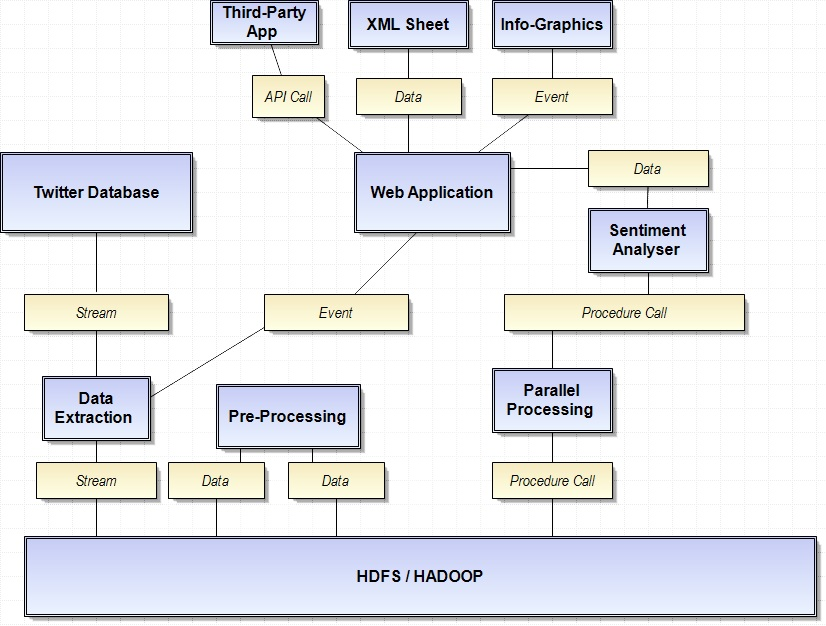
\includegraphics[height=8.5cm]{images/Architecture.jpg}
	\captionof{figure}{SENTAL Architecture}
\end{center}
\section{Data Flow Diagram}
The data flow in the proposed system is shown below with the help of data flow diagram consisting of three levels.\\
\hspace*{\parindent}User and Sentiment Analyzer are two actors and SENTAL system is the main process. The user passes a desired keyword, of which he/she wants the result of, through the interface. This keyword goes to the process SENTAL system, where it gets processed through other actor- Sentiment Analyzer. The sentiment analyzer processes the keyword returned from SENTAL system to produce the result. The analysis result is passed through SENTAL system and returned to the user as a form of infographics or xml sheet.

\subsection{Level 0}
\begin{center}
	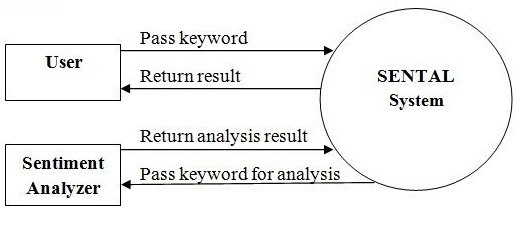
\includegraphics[height=6cm]{images/DFD1.jpg}
	\captionof{figure}{DFD Level 0}
\end{center}
\hspace*{\parindent}The actors in the system are User and Sentiment analyzer. SENTAL System is the process. User interacts with the SENTAL system through the Pass keyword and Return result dataflow. Similarly, Sentiment Analyzer interacts with data source through Return result and Pass keyword.
\subsection{Level 1}
\begin{center}
	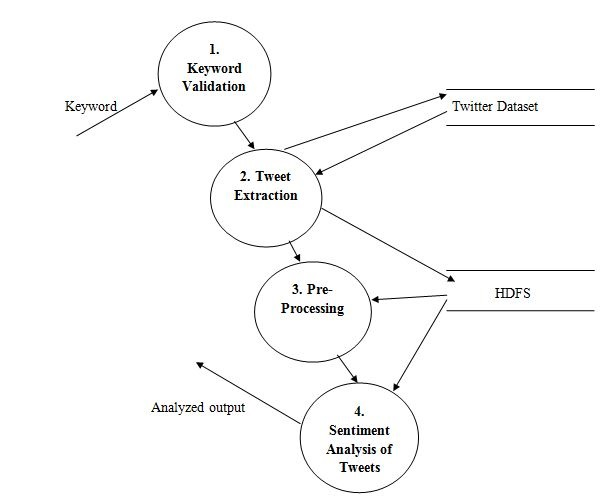
\includegraphics[height=8.5cm]{images/Dfd_level1.jpg}
	\captionof{figure}{DFD Level 1}
\end{center}
\hspace*{\parindent}Entered keyword is validated by Keyword Validation process which is then passed to the Tweet Extraction process. It has access to Twitter dataset data source and HDFS data source. Further pre-processing process gets the raw tweets and gives output to the process Sentiment Analysis as shown in figure 5.2. Analyzed output is given out by the same process.
\subsection{Level 2}
\begin{center}
	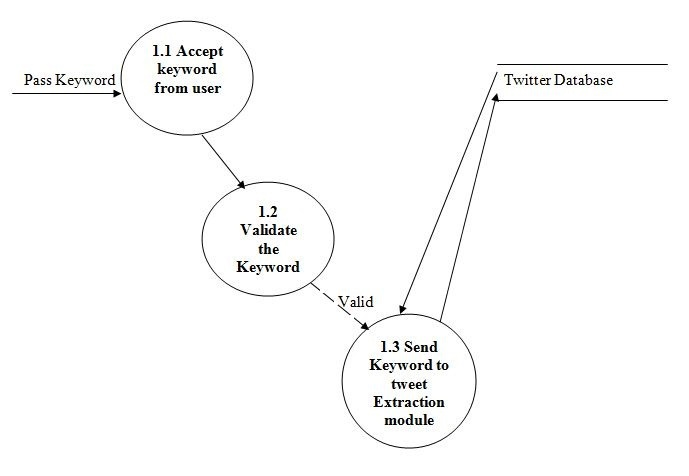
\includegraphics[height=8.1cm]{images/level21.jpg}
	\captionof{figure}{DFD Level 2 for tweets extraction}
\end{center}
\hspace*{\parindent}Process 1.1 accepts the keyword from the user and is passed to the process 1.2 to validate the entered keyword. The keyword marked as validated is then passed to process 1.3 where it sends the valid keyword to Tweet Extraction Module. This process has access to the data store Twitter database.
\begin{center}
	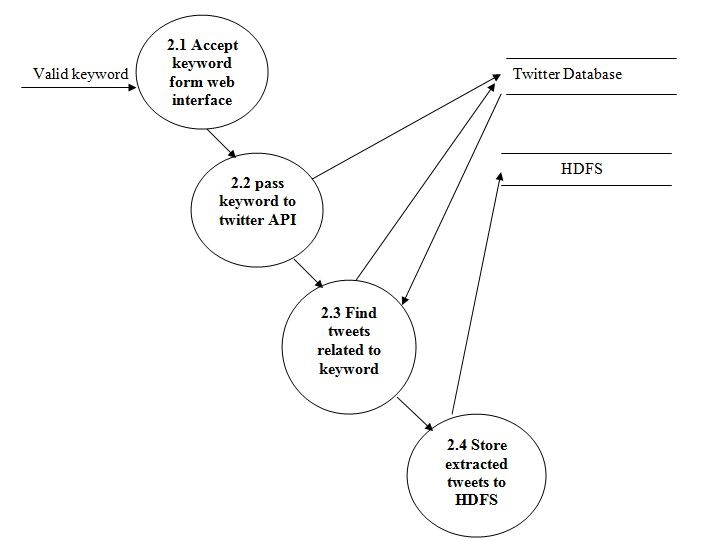
\includegraphics[height=8cm]{images/level22.jpg}
	\captionof{figure}{DFD Level 2 for storing to HDFS}
\end{center}
\hspace*{\parindent}Valid keyword is passed to web interface through process 2.1, and it is transferred to Twitter API through process 2.2. It accesses Twitter Database to find related tweets using the process 2.3. The output of process 2.3 is passed to process 2.4 to store the extracted tweets to HDFS. It uses the data store HDFS as shown in figure 5.
\begin{center}
	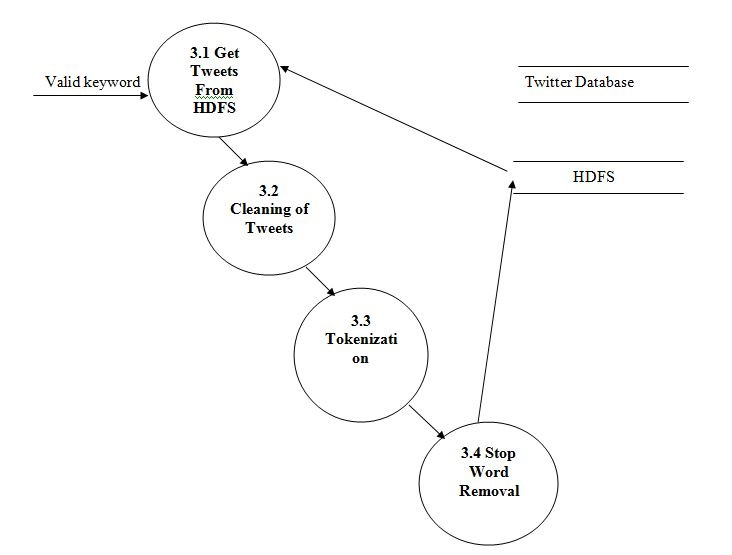
\includegraphics[height=8.5cm]{images/level23.jpg}
	\captionof{figure}{DFD Level 2 for Preprocessing}
\end{center}
\hspace*{\parindent}Process 3.1 gets the tweets that are stored in HDFS. It is then passed to the process 3.2 for the cleaning of tweets, followed by the process 3.3, where the tweets are tokenized. The tokenized tweets are passed to the process 3.4 for the Stop-word removal process. The data store accessed is the HDFS.
\begin{center}
	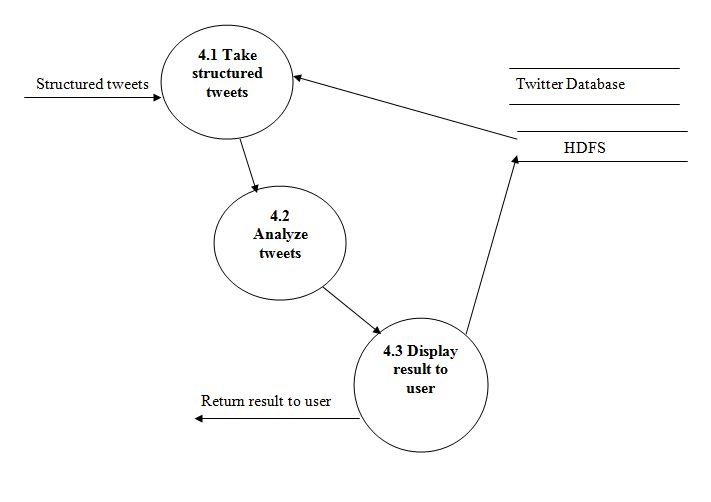
\includegraphics[height=9cm]{images/level24.jpg}
	\captionof{figure}{DFD Level 2 for Sentiment Analyzer}
\end{center}
\hspace*{\parindent}Input to the process 4.1 is the structured tweets, which are sent to the process 4.2, which analyzes the tweets. Output of process 4.2 is sent to process 4.3, which displays the result to the user. The data source used here is HDFS.

\section {UML Diagrams}
\subsection{Use case Diagram}
\begin{center}
	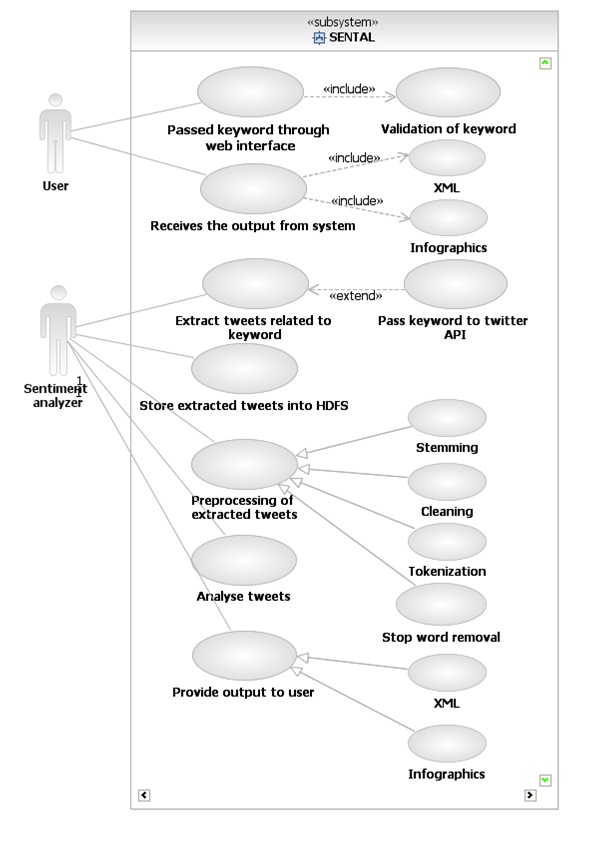
\includegraphics[height=16cm]{images/usecase.jpg}
	\captionof{figure}{Use Case Diagram}
\end{center}
\hspace*{\parindent}The Use case diagram for the proposed system is shown above\\
\hspace*{\parindent} The system has two main actors:\\
\hspace*{\parindent} 1.  User   2. Sentiment Analyzer\\
\hspace*{\parindent} The User and Sentiment Analyzer interact through various use cases. Some of the cases undergo generalization and specialization, and are shown by keywords include and extend respectively.
User passes keyword through the designed web interface. The keyword is validated and result is extracted through sentimental analyzer and result is passed to the user. The sentiment analyzer receives the keyword from the interface and it extracts the various tweets related to the keyword. Part of the sentiment analyzer, processes the extracted tweets, using various processes like stemming, cleaning, tokenization and stop word removal. The output is displayed in the web page in the form of info graphics or xml sheet.

\subsection{Activity Diagram}
\begin{center}
	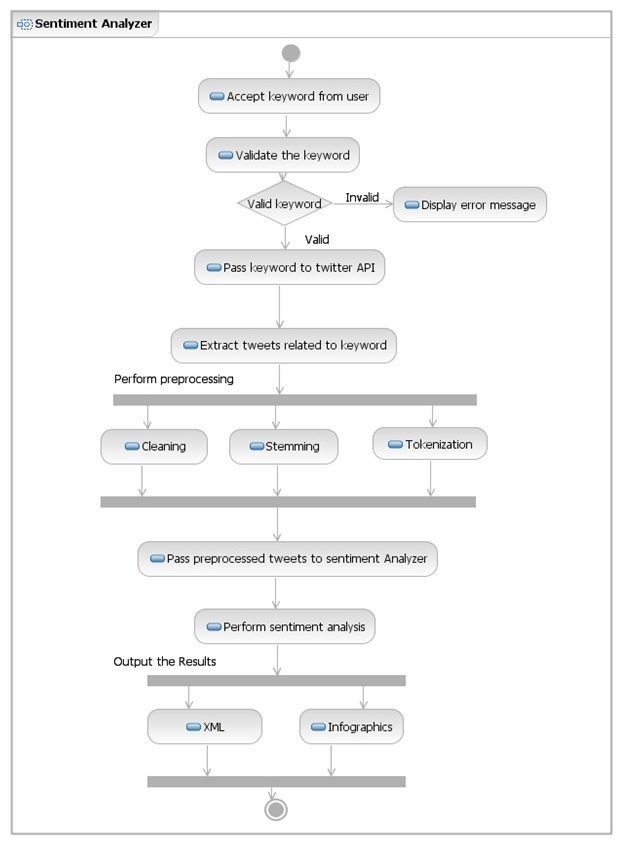
\includegraphics[height=14cm]{images/activity.jpg}
	\captionof{figure}{Activity Diagram}
\end{center}
\hspace*{\parindent}The Activity diagram for the proposed system is shown in above diagram.\\
\hspace*{\parindent}The actor passes a keyword to the web application. The keyword is validated for correct and approved format and the errors are shown, if present. The web application passes the keyword to the twitter database through the sentiment analyzer. The twitter API returns the matched terms for the keyword and returns the raw data to sentiment analyzer. The sentiment analyzer analyses the raw tweets and processes them to produce the result in form of infographics or xml sheet.
\subsection {Sequence Diagram}
\begin{center}
	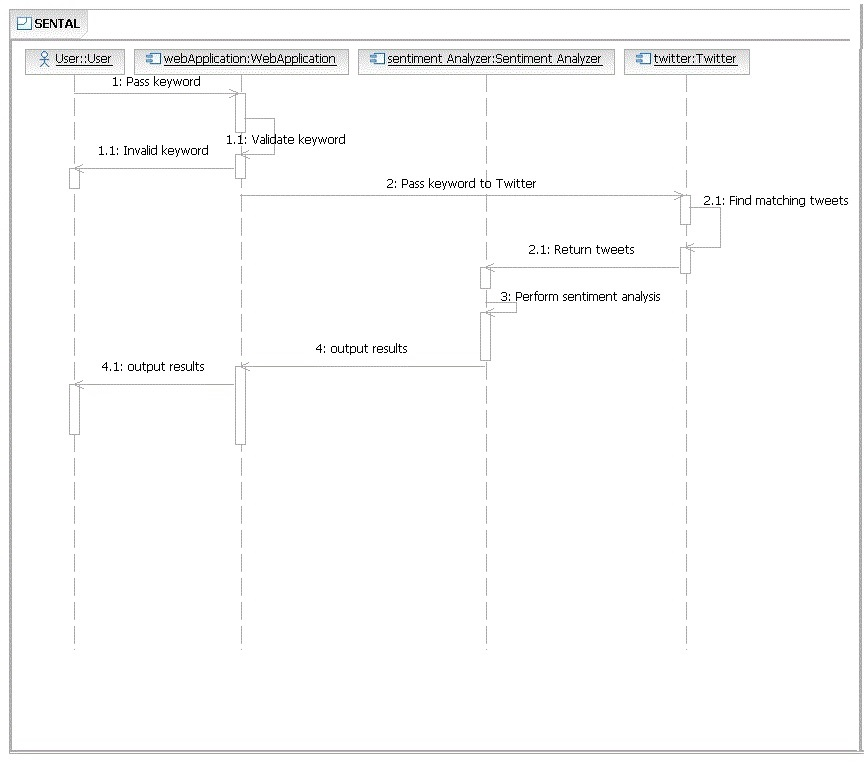
\includegraphics[height=14cm]{images/state.jpg}
	\captionof{figure}{Sequence Diagram}
\end{center}
\hspace*{\parindent}The sequence diagram for the proposed system is as shown in figure 6 diagram.\\
\hspace*{\parindent} The actor here is User. The actor passes a keyword to the web application. The keyword is validated for correct and approved format and the errors are shown, if present.\\
\hspace*{\parindent} The web application passes the keyword to the twitter database through the sentiment analyzer. The twitter API returns the matched terms for the keyword and returns the raw data to sentiment analyzer. The sentiment analyzer analyses the raw tweets and processes them to produce the result in form of infographics or xml sheet.	

\chapter{Implementation Details}
\section{Installation of Cloudera’s Distributed Hadoop}
Installation starts with VMWare and booted it with Cent OS, and then we installed CDH through command line.\\
\hspace*{\parindent}Further installation included following softwares:
\begin{itemize}
	\item MySQL Server
	\item Oracle JDK
	\item Flume, Hive, Oozie
\end{itemize}
After installation, we tested CDH ecosystem as given in figure  below:
\begin{center}
	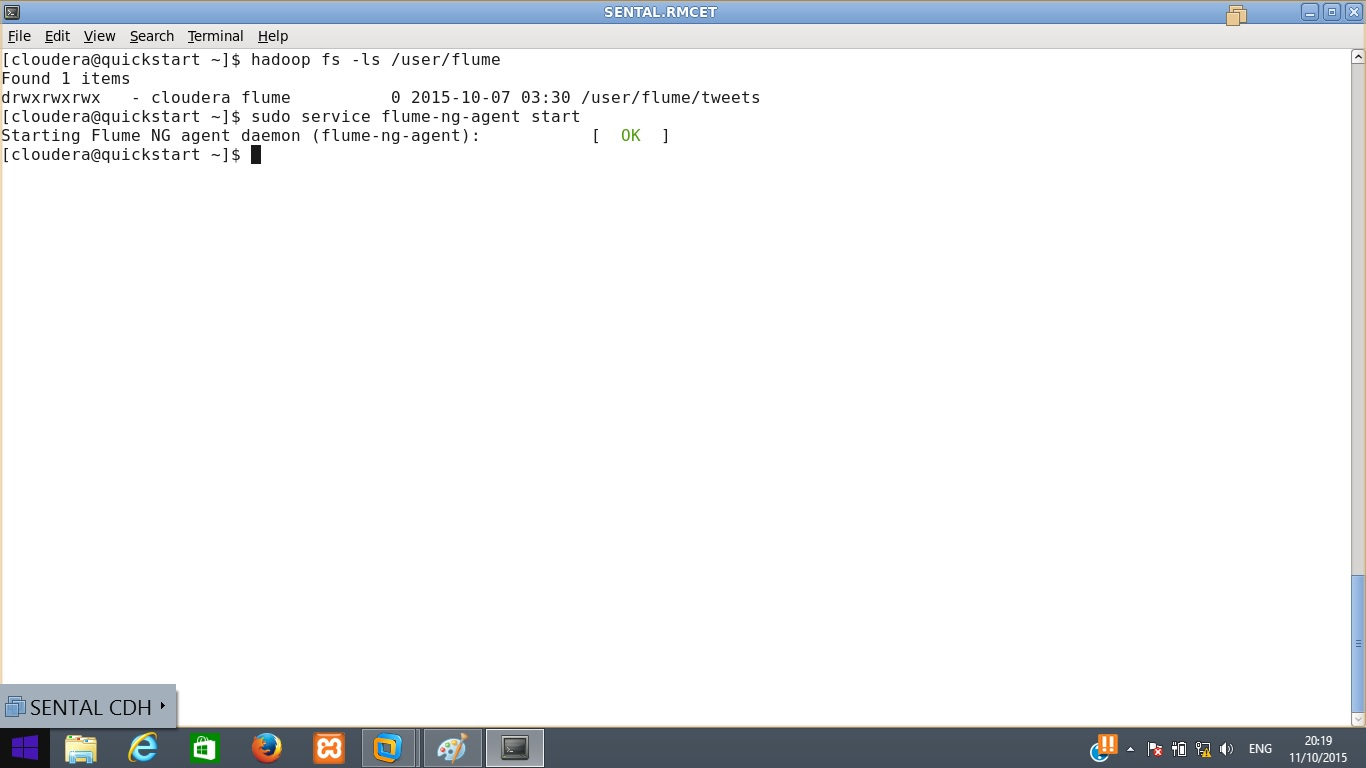
\includegraphics[height=9cm]{images/installation.jpg}
	\captionof{figure}{Installation of Cloudera’s Distributed Hadoop}
\end{center}
\section{Generation of Twitter Stream API Keys}
Created an application named SENTAL.rmcet in https://dev.Twitter.com/apps/ and then generated the corresponding keys.
\begin{center}
	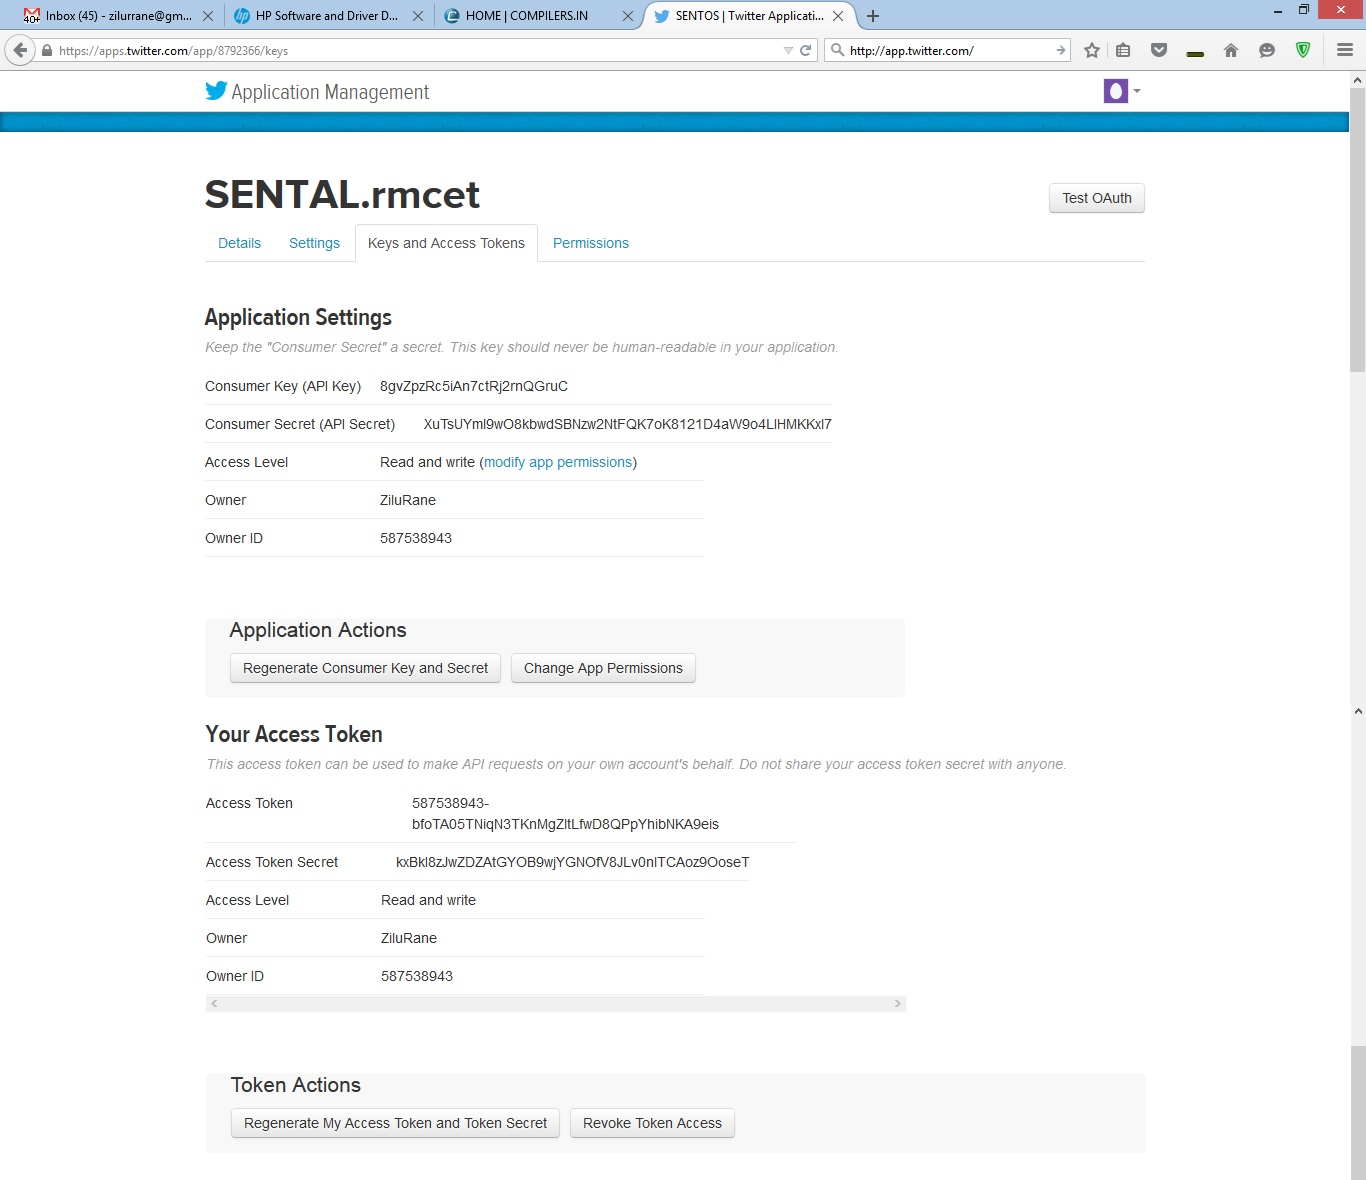
\includegraphics[height=8cm,width=16cm]{images/twitterapi.jpg}
	\captionof{figure}{Generation of Twitter Stream API Keys}
\end{center}
\section{Flume Configuration}
Now we edited /etc/flume.conf file which was previously empty and mentioned keys generated in above step.\\
\hspace*{\parindent} Detailed script is shown in figure. 
\begin{center}
	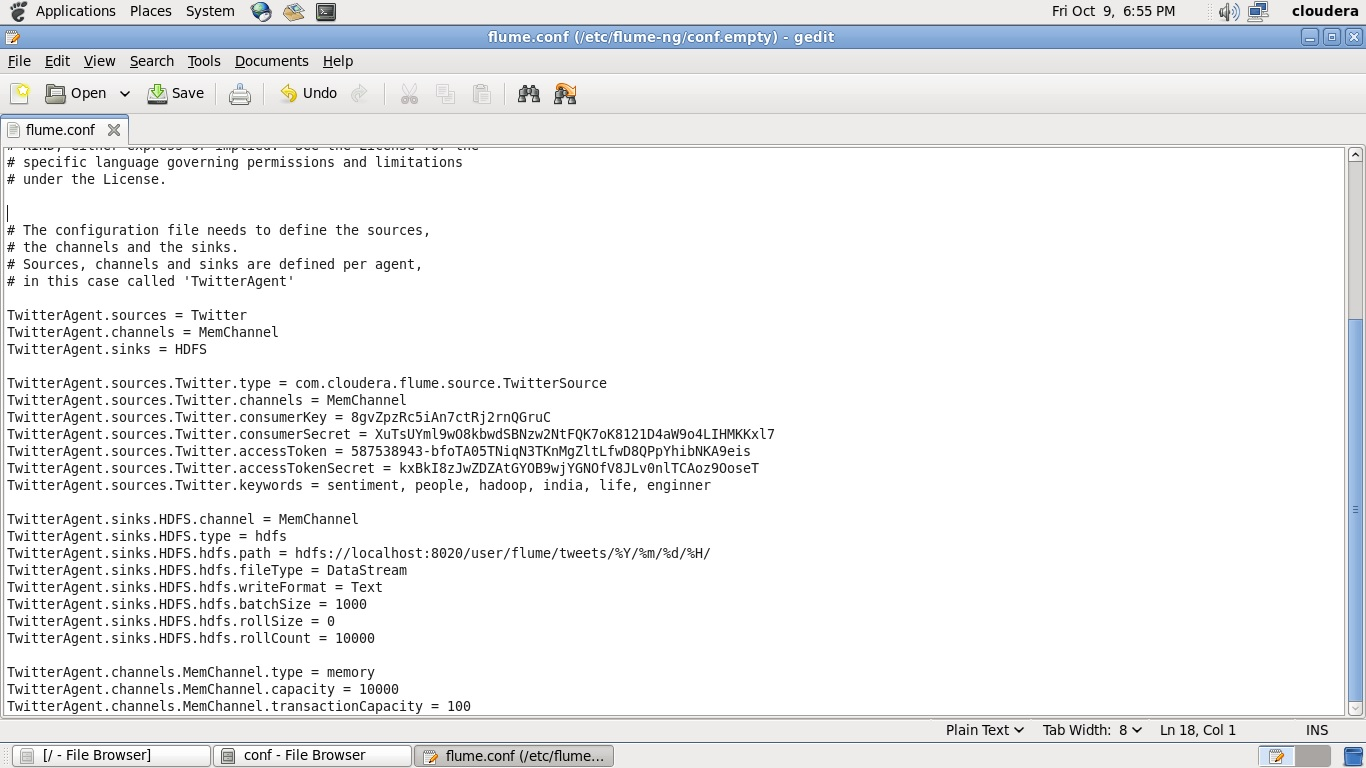
\includegraphics[height=7cm,width=16cm]{images/flume.jpg}
	\captionof{figure}{Flume Configuration}
\end{center}
\section{Design of SENTAL GUI}
\begin{center}
	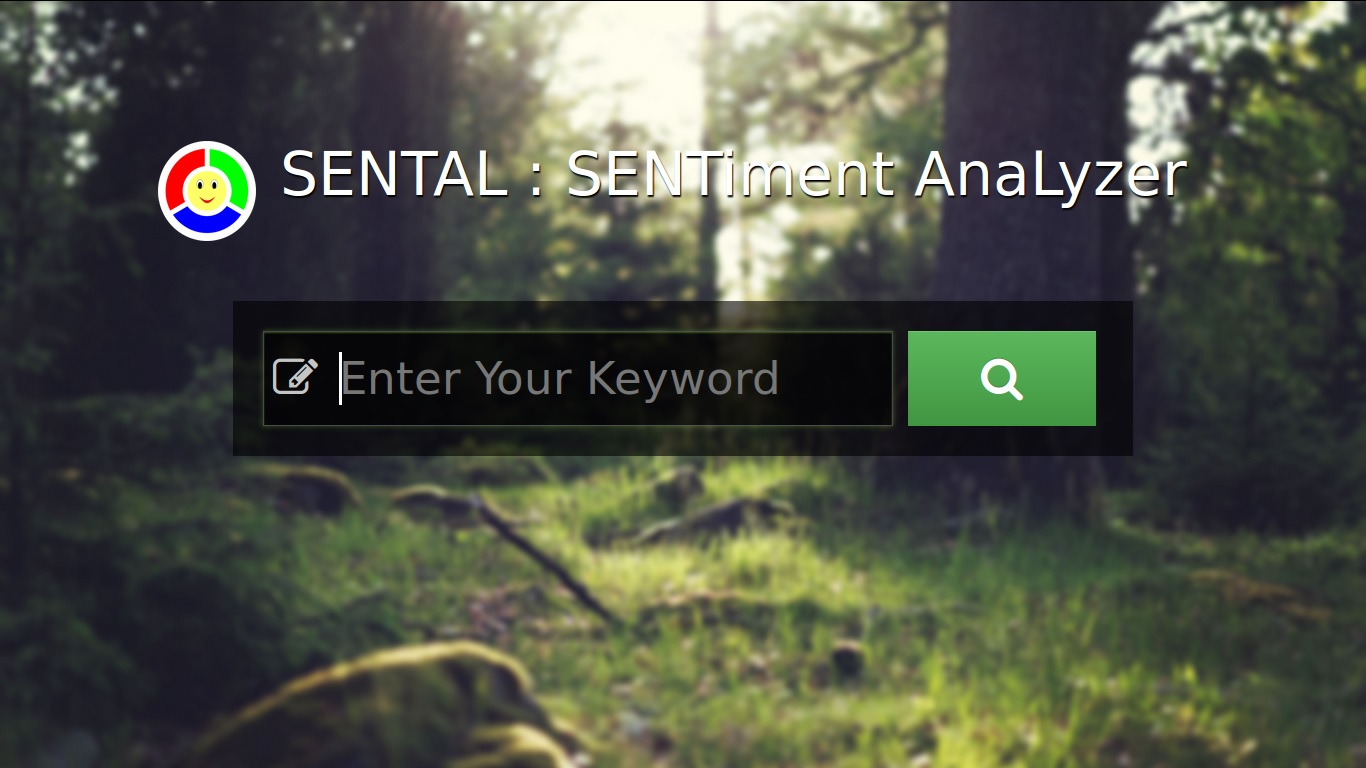
\includegraphics[height=8cm,width=16cm]{images/homepage.jpg}
	\captionof{figure}{SENTAL Homepage}
\end{center}
This is the web interface for user for entering the desired keyword for which he/she is expected to find out the sentiments of.\\ 
\textbf{SENTAL output}
\begin{center}
	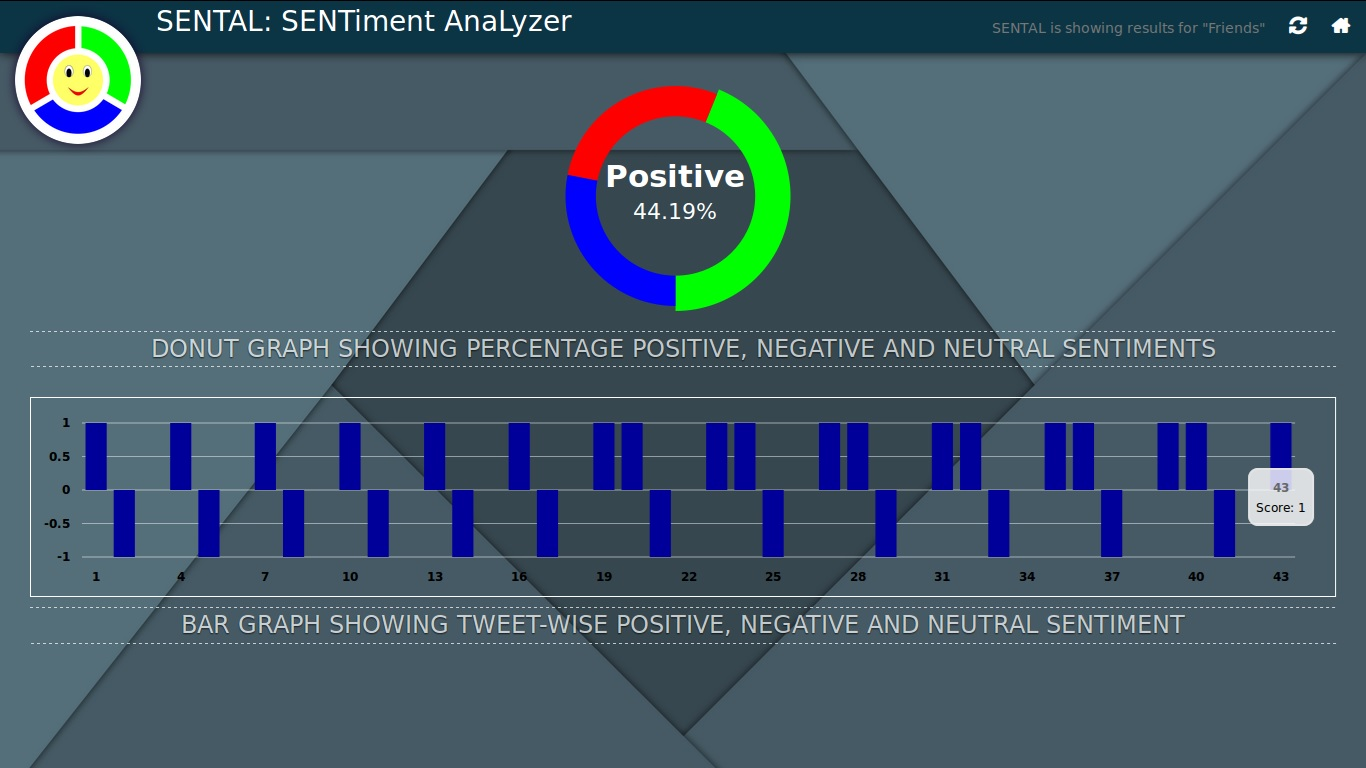
\includegraphics[height=9cm,width=16cm]{images/output.jpg}
	\captionof{figure}{SENTAL output}
\end{center}
This interface displays the sentiments analysed based on the keyword entered by user. The results are displayed in the form of infographics - bar charts and a pie-chart
\section{Design of Algorithm}
\subsection{DATA}
\textbf{Raw Tweets}\\
\hspace*{\parindent}	[4]This dataset is the collection of tweets which are extracted using flume. These tweets are in the unstructured data format. The dataset is full of many non-English words along with technical substitutions. This dataset needs to be prepossessed for the effective analysis. This part is done in Preprocessing module.\\
\hspace*{\parindent}\textbf{Dictionaries }\\
\hspace*{\parindent}	The algorithm maintains dictionaries which are effectively the training sets for the classification purpose. The training set is backbone of the algorithm- more strong the training set, more accurate is the analysis of sentiments.\\
\hspace*{\parindent} The dictionaries we’ve implemented are basically yaml files. It is a markup format used for building up dictionary. There are six main dictionaries built for algorithm. They are:
positive.yml, negative.yml, neutral.yml, inv.yml, inc.yml and dec.yml.
\subsection{PRE-PROCESSING}
\hspace*{\parindent}Due to the varying and unpredictable nature of language used in tweets, it is likely that preprocessing mechanism [5] could be used to standardize certain tokens of tweets. It is highly likely that most tweets contain some form of acronym, grammatical or spelling mistakes, colloquialisms and slangs; incorporated into due to the 10,000-character limit imposed by Twitter on tweets.\\
\hspace*{\parindent}The quality of the data affects the results and therefore in order to improve the result, the raw data is pre-processed. It deals with the preparation that removes the repeated words and punctuations and improves the efficiency of analysis algorithms.\\
\hspace*{\parindent} The pre-processing module extracts the relevant content from the tweets while leaving out the irrelevant ones. The techniques applied in this paper are used commonly in information retrieval applications specifically in sentiment analysis in micro-blogging. The collected data is passed through a series of pre-processors.\\
\hspace*{\parindent} Some of the pre-processing steps that have been carried out are explained below.: 
\begin{center}
	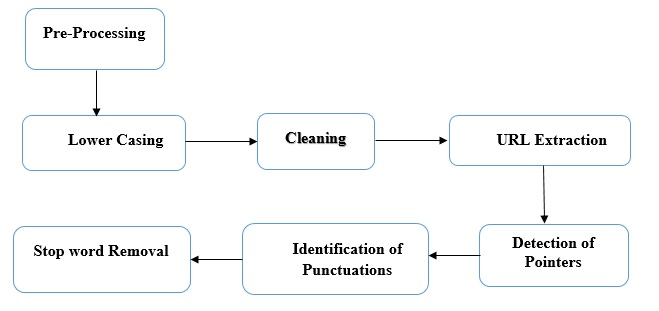
\includegraphics[height=7cm,width=16cm]{images/processingmoldule.jpg}
	\captionof{figure}{Pre-processing Module}
\end{center}
\textbf{Lower Casing }\\
\hspace*{\parindent} It is important to have the entire word in a consistent case when classifying texts in order to guarantee that all tokens map to the corresponding feature irrespective of casing.[6] This is extremely important for this research work as it is very common to find irregular casing(such as "TwITteRseNtlMeNtanAIYsiS") in micro-blogs.\\
\newline
\textbf{Cleaning}\\
\hspace*{\parindent}By using a list of cut off patterns, we omit contact addresses and formatting in order to extract only the[6] textual components, smileys,\\
\newline
\textbf{URL Extraction}\\
\hspace*{\parindent}Many tweets contain URLs in order to share more content than what can be given in the limited-character post. The content in the URL might provide supplementary knowledge regarding the emotion a user trying to express, however it would be far too expensive to crawl URLs for their content. In order to trim down the feature size during training, all URLs in the training tweets have been replaced with an equivalence class  URL. This could considerably reduce feature size.\\
\newline
\textbf{Detection of Pointers }\\
\hspace*{\parindent} In Twitter, posts can point to other users with the use of and @ token in front of a username. And users tag tweets pertaining to a category in twitter, using \#. Again, to avoid explosion of features, we abstract it to a constant symbol  USER and  HASHTAG. This replacement of usemames and hashtags reduce the feature size by a large margin.\\
\newline
\textbf{Identification of Punctuations}\\ 
\hspace*{\parindent} In micro-blogging space, it is common to use excessive punctuation in order to stay away from proper grammar and to communicate emotion more easily. The punctuations can also give insight to the polarity of the message. For example, exclamation marks are used to express powerful emphasis which are usually polar messages [13]. In this step, irrelevant punctuations marks were removed by replacing PUNCT  to avoid redundant feature in the training set.\\
\newline
\textbf{Stop word Removal  }\\ 
\hspace*{\parindent}Words without a deeper meaning, such as the, is, of, are named [7]stop words and can thus be removed. We use a list of stop words.
\begin{center}
	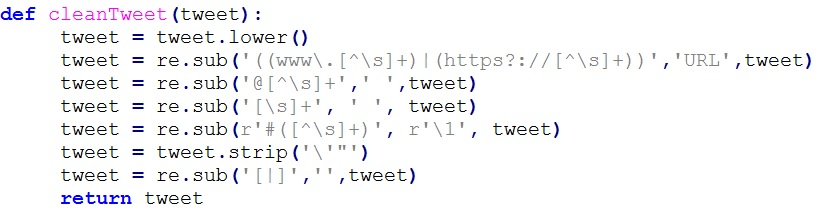
\includegraphics[height=4cm]{images/codepreprocessing.jpg}
	\captionof*{figure}{PRE-PROCESSING MODULE}
\end{center}

\subsection{TOKENIZATION  MODULE}
\hspace*{\parindent}We segment tweets by splitting it by spaces and punctuation marks, and form a bag of words. [7]That is each tweet is split into sentences and single words named tokens.
\begin{center}
	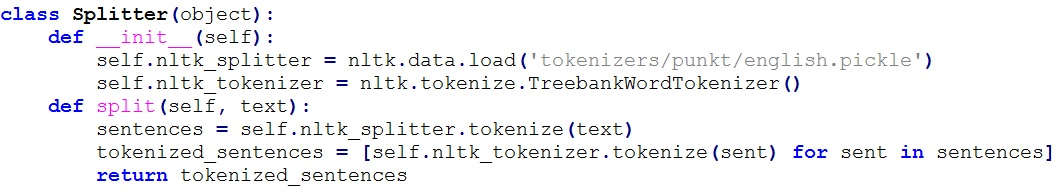
\includegraphics[height=3.2 cm]{images/SplitterModule.jpg}
	\captionof*{figure}{TOKENIZATION  MODULE}
\end{center}

\subsection{PART-OF-SPEECH TAGGING}
One of the earliest steps in the processing of natural language text is part of speech (POS) tagging. Usually this is a sentence-based process and given a sentence formed of a sequence of words, part-of-speech tagging tries to label (tag) each word with its correct part of speech.\\
\hspace*{\parindent}The mechanism of classifying words into their parts of speech and labeling them accordingly is known as part-of-speech tagging, POS-tagging, or simply tagging. Parts of speech are also known as word classes or lexical categories. The collection of tags used for a particular task is known as a tag set.\\
\hspace*{\parindent}A part-of-speech tagger, or POS-tagger, processes a sequence of words, and attaches a part of speech tag to each word:
\begin{center}
	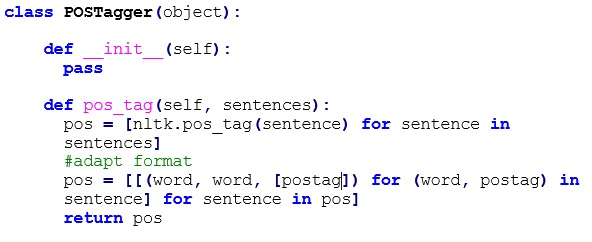
\includegraphics[height=6cm]{images/codeposttagging.jpg}
	\captionof*{figure}{PART-OF-SPEECH TAGGING  MODULE}
\end{center}
\subsection{DICTIONARY TAGGING}
\hspace*{\parindent} Dictionary tagging is implemented by dict tagger module. The sole purpose of dictionary tagging is to lookup for the arrival of tokenised word in the predefined training sets.\\
\hspace*{\parindent} Initially, it opens all the dictionaries and keep them ready for mapping. The lookup of the extracted token is then followed in every opened dictionary. As soon as the token is found in either of the dictionaries, the tagger notifies the presence of the token in corresponding dictionary. After successfully tagging, it returns tagged sentences.\\ 
\textbf{Lemmatization }\\ 
\hspace*{\parindent}	In computational linguistics, stemming refers to the process that reduces inflected words to their stem. This process is carried out by the lemmatiser() module. The lemmatisation results in the drawing out a derived word to it’ s root form. This is an important step in NLP.
\begin{center}
	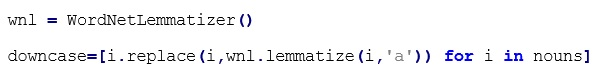
\includegraphics[height=2cm]{images/codelemmatize.jpg}
\end{center}
\textbf{Calculation of Sentence Score }\\ 
\hspace*{\parindent}In this module, following dictionaries serve the most important role of calculating sentiment score:- inc.yml, dec.ml and inv.yml.\\
\hspace*{\parindent}If a tagged token is found to be of positive sentiment, the score is added multiplicatively. On contrast, if the token is found as of negative sentiment, the score is subtracted divisionally. If word  which changes the polarity of a sentence are encountered, then the token is looked up in inv.yml dictionary and the score is inverted multiplicatively.
\begin{center}
	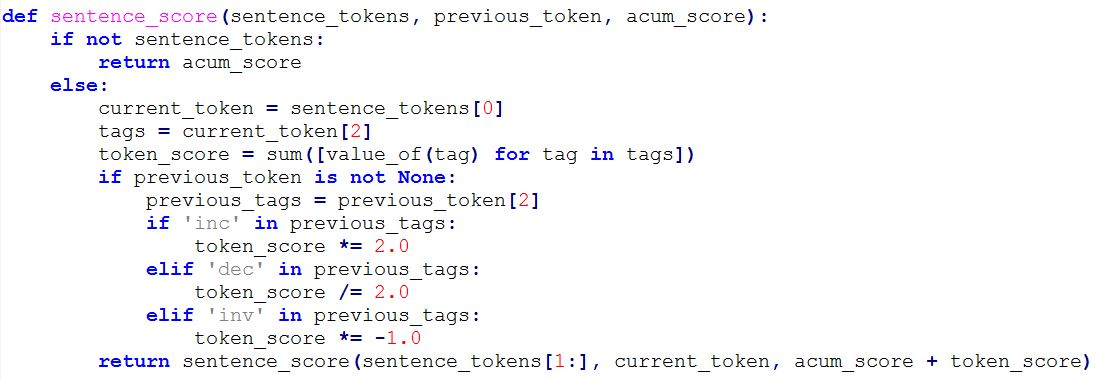
\includegraphics[height=6cm]{images/SentenceScoreModule.jpg}
	\captionof*{figure}{SCORE CALCULETION MODULE}
\end{center}
\textbf{Storing of Result}\\ 
\hspace*{\parindent}	Finally, overall sentiment score of a tweet is calculated and is stored in a separate output file. This file is an input for the Graph Rendering module, which renders an infographic format of sentiment analysis.\\
\textbf{Consider a sample tweet to be analyzed }
\begin{center}
	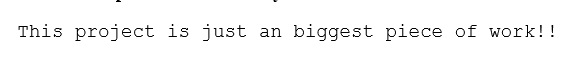
\includegraphics[height=1.5cm]{images/1.jpg}
\end{center}
The first step carried out is the tokenisation of the sentence.
\begin{center}
	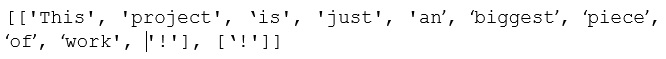
\includegraphics[height=1.4cm]{images/2.jpg}
\end{center}
\hspace*{\parindent}The tokenized words are stored in a list in python.\\
\hspace*{\parindent}The second step is to convert the tokens to possible root word by lemmatizer() function:
\begin{center}
	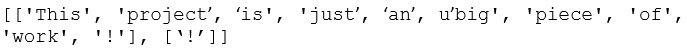
\includegraphics[height=1.1cm]{images/3.jpg}
\end{center}
\hspace*{\parindent}In next step, every token undergoes part of Speech tagging by POSTagger module:
\begin{center}
	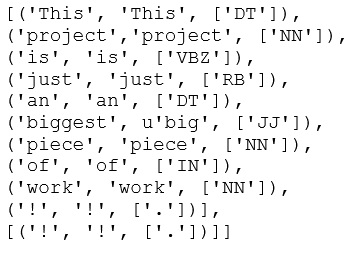
\includegraphics[height=6cm]{images/4.jpg}
\end{center}
\hspace*{\parindent}Then the POSTagged tokens are looked up in dictionaries or training set to find out it’s sentiment.
\begin{center}
	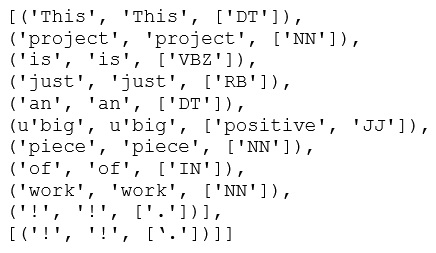
\includegraphics[height=6cm]{images/5.jpg}
\end{center}
\hspace*{\parindent}Once the tokens are successfully classified by the algorithm, a sentiment score is calculated for whole sentence:
\begin{center}
	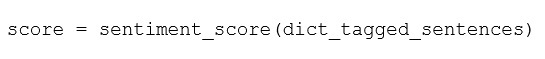
\includegraphics[height=1.5cm]{images/6.jpg}
\end{center}
\hspace*{\parindent}The value of a score is either positive or negative or 0 Accordingly the newly arrived token is added to the corresponding dictionary.\\
\hspace*{\parindent}Finally, the overall result for the score is stored to a text file name Result-Tweets.txt.\\
This file serves as an input to the graph rendering module.


\chapter{Technology Used}
\section{Python}
Python is a multi-paradigm programming language: object-oriented programming and structured programming are fully supported, and there are a number of language features which support functional programming and aspect-oriented programming (including by metaprogramming and by magic methods) Many other paradigms are supported using extensions, including design by contract and logic programming. \\
\hspace*{\parindent}Python uses dynamic typing and a combination of reference counting and a cycle-detecting garbage collector for memory management. An important feature of Python is dynamic name resolution (late binding), which binds method and variable names during program execution. The design of Python offers some support for functional programming in the Lisp tradition. The language has map(), reduce() and filter() functions; comprehensions for lists, dictionaries, and sets; and generator expressions. The standard library has two modules (itertools and functools) that implement functional tools borrowed from Haskell and Standard ML\\
\hspace*{\parindent}Python has a large standard library, commonly cited as one of Python's greatest strengths, providing tools suited to many tasks. This is deliberate and has been described as a "batteries included" Python philosophy. For Internet-facing applications, a large number of standard formats and protocols (such as MIME and HTTP) are supported. Modules for creating graphical user interfaces, connecting to relational databases, pseudorandom number generators, arithmetic with arbitrary precision decimals, manipulating regular expressions, and doing unit testing are also included.\\
\hspace*{\parindent}	Most Python implementations (including CPython) can function as a command line interpreter, for which the user enters statements sequentially and receives the results immediately (REPL). In short, Python acts as a shell.
Other shells add capabilities beyond those in the basic interpreter, including IDLE and IPython. While generally following the visual style of the Python shell, they implement features like auto-completion, retention of session state, and syntax highlighting.
\section{Hadoop}
\textbf{HADOOP ARCHITECTURE  }\\ 
\hspace*{\parindent}Hadoop make use of HDFS for data storage purpose. Each cluster of Hadoop contains variety of nodes hence HDFS architecture is broadly divided into following three nodes,
\begin{itemize}
	\item Name Node.
	\item Data Node.
	\item HDFS Clients(Edge Node).
\end{itemize}
\begin{center}
	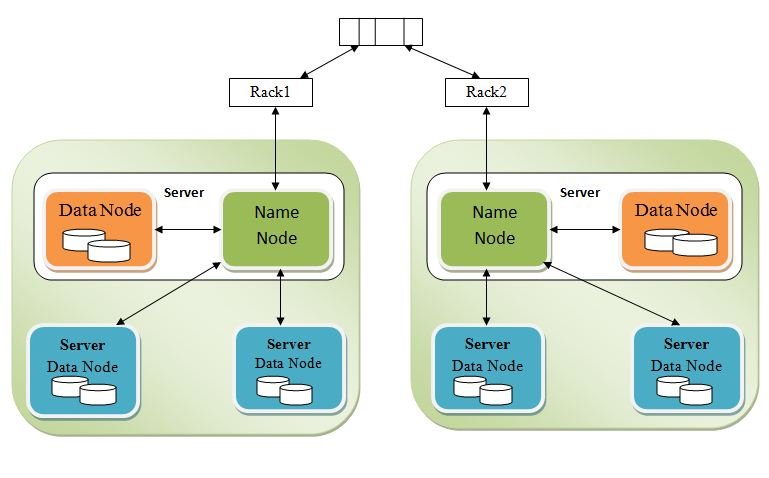
\includegraphics[height=5.8cm]{images/architectureHadoop.jpg}
	\captionof{figure}{Hadoop Architecture}
\end{center}
\textbf{Name Node: }\\ 
\hspace*{\parindent}Name Node is also known as master node, which contains the information about or we can say that meta data about the all data node and there address(use to talk ), free space, data they store, active data node , passive data node, task tracker, job tracker and many other configuration like  replication of data.\\
\textbf{Data Node: }\\
\hspace*{\parindent}In simple words, Data Node is one type of slave node in the Hadoop, which is used to save the data and there is task tracker in data node which is use to track on the ongoing job on the data node and the jobs which coming from name node.\\
\textbf{HDFS Clients: }\\ 
\hspace*{\parindent}Hadoop Architecture, is based on HDFS, which is hadoop distributed file system. In which data is equally (ideally) distributed on each node in the hadoop system. When client want to fetch or add or modify or delete some data from hadoop, then hadoop system collect the data from each node and do the meaningful actions as per requirement.

\chapter{Test Cases}
\newpage
\begin{table}[ht!]
\centering
\caption{Test Cases}
\label{my-label}
\resizebox{\textwidth}{!}{%
\begin{tabular}{@{}|c|c|c|c|c|c|c|c|@{}}


\cline{1-8}
\multicolumn{4}{|c|}{\Large \textbf{Test Cases}} & \multicolumn{4}{c|}{\Large \textbf{ Test Steps}} \\
\cline{1-8}
\large \textbf{Sr. No.} & \large \textbf{ID} & \large \textbf{Test Case Name} & \large \textbf{Test Case Description} & \large \textbf{Step} & \large \textbf{Expected Result} & \large \textbf{Actual Result} & \large \textbf{Status} \\
\cline{1-8}
\multicolumn{1}{|c|}{1} & \multicolumn{1}{c|}{TC001} & \multicolumn{1}{l|}{Preprocessing} & \multicolumn{1}{l|}{\begin{tabular}[c]{@{}l@{}}Passing raw unstructured tweets\\to Cleaning module and\\ getting cleaned tweets\end{tabular}} & \multicolumn{1}{c|}{\#1} & \multicolumn{1}{c|}{Preprocessed tweets} & \multicolumn{1}{c|}{As expected} & \multicolumn{1}{c|}{Pass} \\
\cline{1-8}
\multicolumn{1}{|c|}{2} & \multicolumn{1}{c|}{TC002} & \multicolumn{1}{l|}{Tokenization} & \multicolumn{1}{l|}{\begin{tabular}[c]{@{}l@{}}Splitting individual\\ tweets to tokenss\end{tabular}} & \multicolumn{1}{c|}{\#2} & \multicolumn{1}{c|}{Tokenized tweets} & \multicolumn{1}{c|}{As expected} & \multicolumn{1}{c|}{Pass} \\ \cline{1-8}
\multicolumn{1}{|c|}{3} & \multicolumn{1}{c|}{TC003} & \multicolumn{1}{l|}{POStagging} & \multicolumn{1}{l|}{\begin{tabular}[c]{@{}l@{}}Getting part of speech of\\ each tokens\end{tabular}} & \multicolumn{1}{c|}{\#3} & \multicolumn{1}{c|}{POSTagged tweet} & \multicolumn{1}{c|}{As expected} & \multicolumn{1}{c|}{Pass} \\ \cline{1-8}
\multicolumn{1}{|c|}{4} & \multicolumn{1}{c|}{TC004} & \multicolumn{1}{l|}{Dictionary Tagging} & \multicolumn{1}{l|}{\begin{tabular}[c]{@{}l@{}}Looking up the training set\end{tabular}} & \multicolumn{1}{c|}{\#4} & \multicolumn{1}{c|}{Dictionary tagged tokens} & \multicolumn{1}{c|}{As expected} & \multicolumn{1}{c|}{Pass} \\ \cline{1-8}
\multicolumn{1}{|c|}{5} & \multicolumn{1}{c|}{TC005} & \multicolumn{1}{l|}{Score Calculation} & \multicolumn{1}{l|}{\begin{tabular}[c]{@{}l@{}}Calculate score of sentence,\\ to decide whether it is positive,\\ ngative or neutral\end{tabular}} & \multicolumn{1}{c|}{\#5} & \multicolumn{1}{c|}{Accumulated score} & \multicolumn{1}{c|}{As expected} & \multicolumn{1}{c|}{Pass} \\ \cline{1-8}
\multicolumn{1}{|c|}{6} & \multicolumn{1}{c|}{TC006} & \multicolumn{1}{l|}{Main Result storing} & \multicolumn{1}{l|}{\begin{tabular}[c]{@{}l@{}} Storing result of tweet in\\Result-tweet.txt\end{tabular}} & \multicolumn{1}{c|}{\#6} & \multicolumn{1}{c|}{Score get stored in file} & \multicolumn{1}{c|}{As expected} & \multicolumn{1}{c|}{Pass} \\ \cline{1-8}
\multicolumn{1}{|c|}{7} & \multicolumn{1}{c|}{TC007} & \multicolumn{1}{l|}{Dictionary Updating} & \multicolumn{1}{l|}{\begin{tabular}[c]{@{}l@{}}Update dictionary with\\ new training data\end{tabular}} & \multicolumn{1}{c|}{\#7} & \multicolumn{1}{c|}{Updated dictionary} & \multicolumn{1}{c|}{As expected} & \multicolumn{1}{c|}{Pass} \\ \cline{1-8}


\end{tabular}%
}
\end{table}
{\bfseries Note:} \# - Refer appendix
\chapter{Project Timeline}
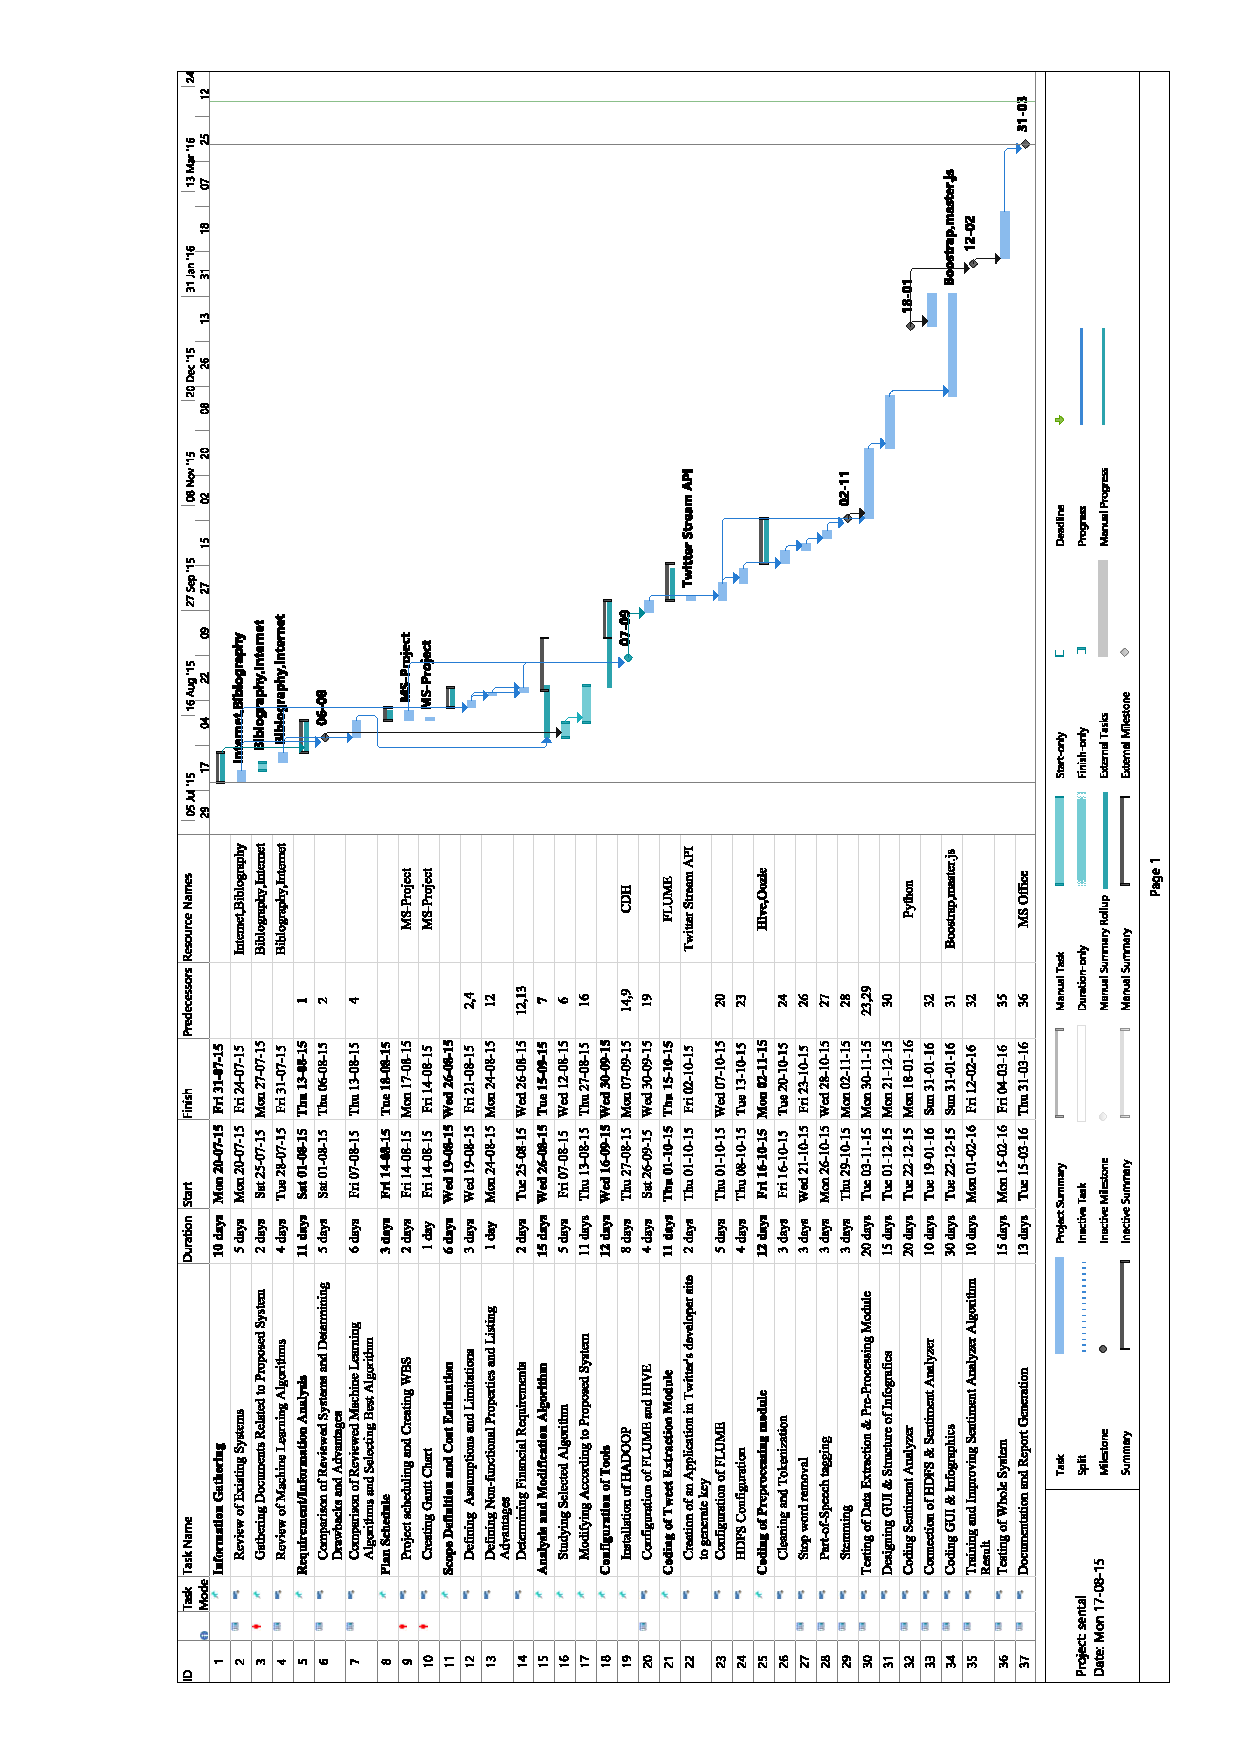
\includepdf[pages={1}]{sentalwbss.pdf}
\chapter{Task Distribution}
\begin{table}[h]
\centering
\caption{Task Distribution}
\label{tab:}
\begin{longtable}{|c|c|c|c|c|c|}
\cline{1-6}
\multirow{2}{*}{Sr. No.} & \multicolumn{2}{c|}{\multirow{2}{*}{Task}} & \multicolumn{3}{c|}{Project Member}\\
\cline{4-6}
& \multicolumn{2}{c|}{}& Zilu & Mayur & Akshay \\%% Use of parbox is interesting too \parbox[t]{2cm}{Text\\Text}
\cline{1-6}
\multirow{2}{*}{1} & \multirow{2}{*}{Requirement Gathering} & Literature Survey & 30\% & 40\% & 30\%\\
\cline{3-6}
 & & Study of Existing Systems & 30\% & 30\% & 40\%\\
\cline{1-6}
\multirow{2}{*}{2} & \multirow{2}{*}{Requirement Analysis} & Distribution of Workload & 40\% & 30\% & 30\%\\
\cline{3-6}
 & & Defining Scope of the Project & 40\% & 30\% & 30\%\\
\cline{1-6}
3 & \multicolumn{2}{c|}{Design} & 40\% & 30\% & 30\%\\
\cline{1-6}
4 & \multicolumn{2}{c|}{Coding and Implementation} & 30\% & 40\% & 30\%\\
\cline{1-6}
5 & \multicolumn{2}{c|}{System Maintenance and Documentation} & 30\% & 30\% & 40\%\\
\cline{1-6}

\end{longtable}
\end{table}
\chapter{Conclusion and Future Work}
	\section{Conclusion}
	Thus, in proposed system we are using a set of techniques of machine learning for sentimental analysis based on Twitter data. We are gathering the Twitter dataset through Hadoop and to analyze content using byes technique to support neutral class.
	\section{Future Work}
	We are going to implement following improvements in future:
	\begin{enumerate}
		\item Provision of API extension in format of XML.
		\item Providing real time simulation of tweet analysis.
		\item Current system is only restricted to Web platform, In future we can extent its scope to mobile platforms like Android apps.
	\end{enumerate}
\begin{thebibliography}{9}
\bibitem{latexcompanion} 
P.D. Turney
\textit{Thumbs Up or Thumbs Down? Semantic Orientation Applied to Unsupervised Classification of Reviews}. 
[\textit{Proceedings of the 40th Annual Meeting of the Association for Computational Linguistics (ACL)}].
Philadelphia, pp. 417-424,
\textit  July 2002.

 
\bibitem{latexcompanion} 
A. Go, R. Bhayani, and L. Huang
\textit{Twitter Sentiment Classification using Distant Supervision}. 
[\textit{Stanford}].
Technical,
\textit  2009.

\bibitem{latexcompanion} 
Balakrishnan Gokulakrishnan
\textit{Opinion Mining and Sentiment Analysis on a Twitter DataStream}. 
[\textit{The International Conference on Advances in ICT for Emerging Regions ICTer 2012: 182-188}].


\bibitem{latexcompanion} 
Ana C.E.S.Lima
\textit{Automatic Sentiment Analysis of Twitter Message}. 
[\textit{2012 Fourth International Conference on Computational Aspects of Social Networks (CASoN)}].
\textit  2012.

\bibitem{latexcompanion} 
K.P.Murphy
\textit{Naive Bayes classifiers}. 
[\textit{Stanford}].
Technical,
\textit  2009.

\bibitem{latexcompanion} 
A. Go, R. Bhayani, and L. Huang
\textit{Twitter Sentiment Classification using Distant Supervision}. 
[\textit{http://www.cs.ubc.cal-murphyk/TeachinglCS340-Fall06/readingiNB.pdf.}].

\bibitem{latexcompanion} 
A. Pak and P.Paroubek
\textit{Twitter as a Corpus for Sentiment Analysisand Opinion Mining}. 
[\textit{Conference on International Language Resources and Evaluation LREC'lO}].
\textit May 2010

\end{thebibliography}
\newpage
\pagestyle{empty}
\addcontentsline{toc}{chapter}{Appendix}
\begin{appendices}
\begin{center}
\begin{bf}
\Huge{Appendix}
\end{bf}
\end{center}
\textbf{\large \#1 : Processing Raw Tweets }
\begin{center}
	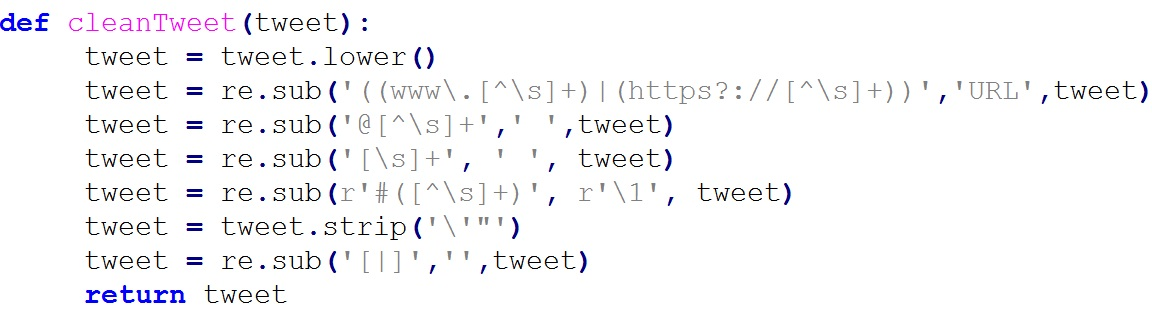
\includegraphics[height=4cm]{images/CleannigTweet_module.jpg}
\end{center}
\textbf{\large \#2 : Tokenization }
\begin{center}
	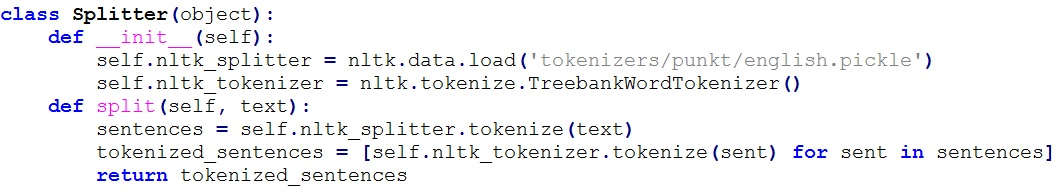
\includegraphics[height=3cm]{images/SplitterModule.jpg}
\end{center}
\textbf{\large \#3 : Part of speech tagging }
\begin{center}
	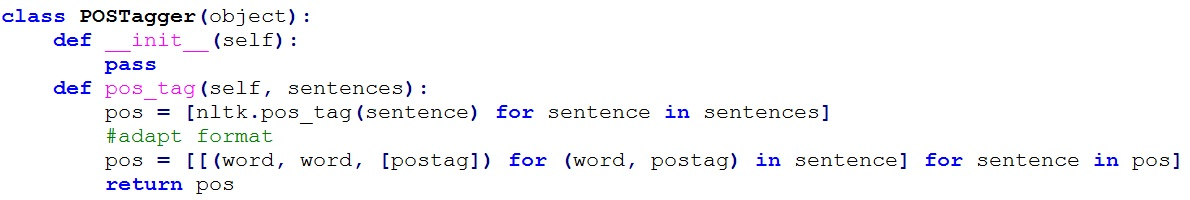
\includegraphics[height=3cm]{images/PostTaggingModule.jpg}
\end{center}
\textbf{\large \#4 : Calculation of sentence score }
\begin{center}
	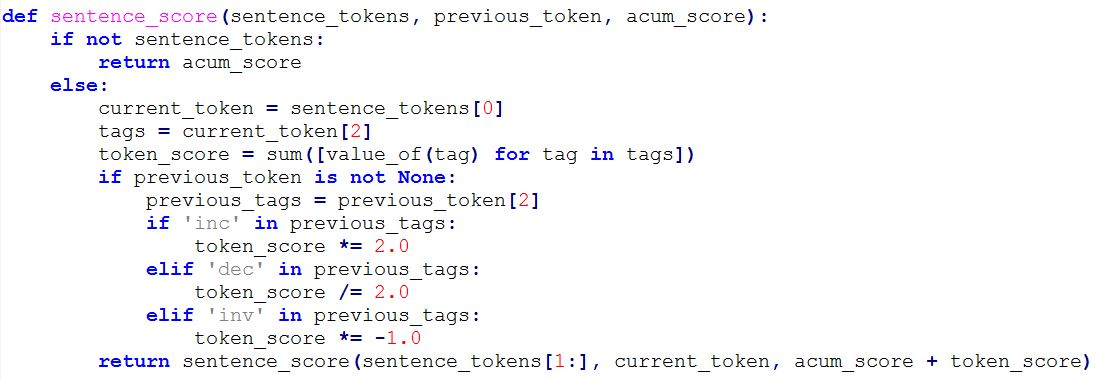
\includegraphics[height=6cm]{images/SentenceScoreModule.jpg}
\end{center}
\textbf{\large \#5 : Dictionary tagging }
\begin{center}
	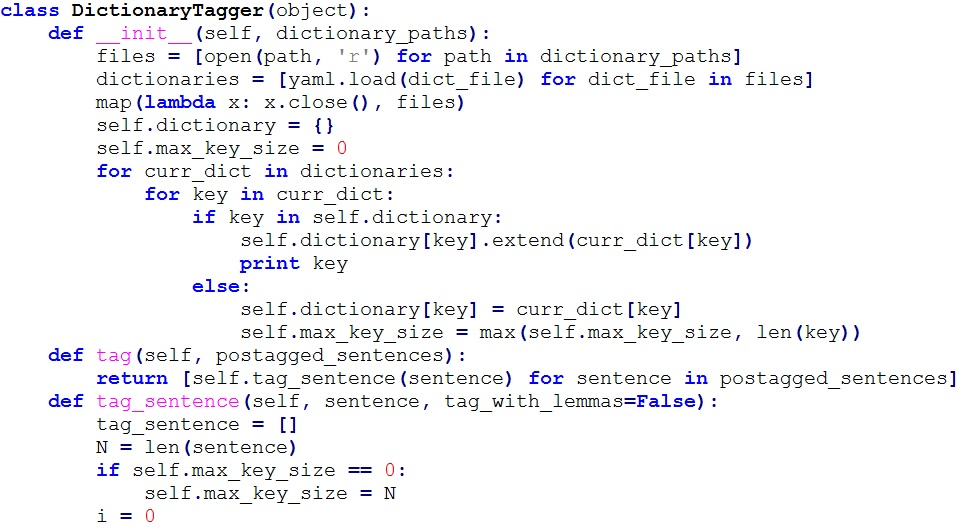
\includegraphics[height=9cm]{images/DicTagging_1.jpg}
\end{center}
\begin{center}
	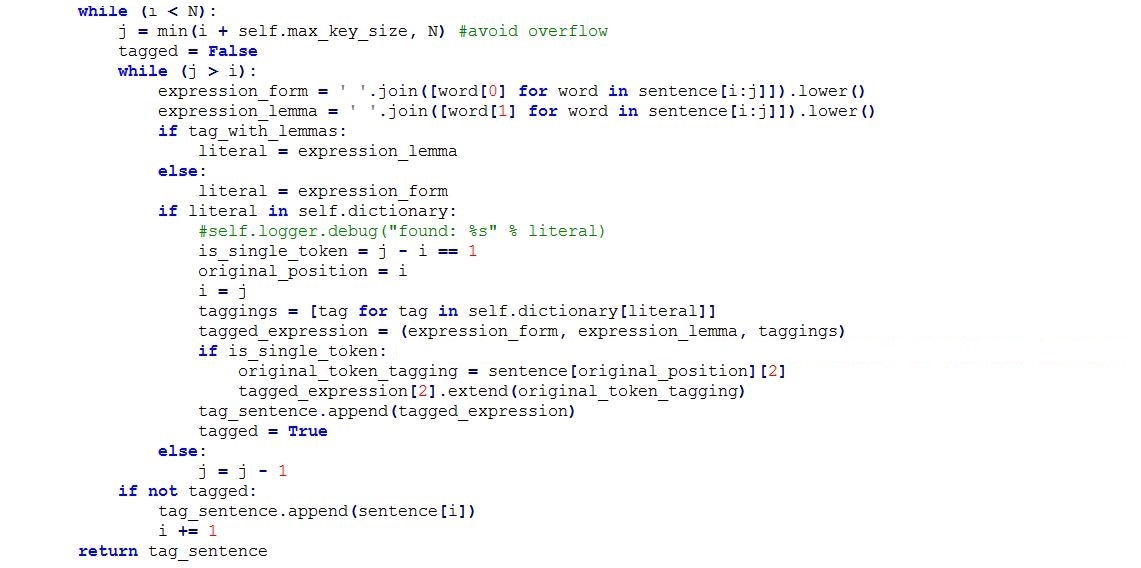
\includegraphics[height=11cm]{images/DicTagging_2.jpg}
\end{center}
\newpage
\textbf{\large \#6 : Main result storing }
\begin{center}
	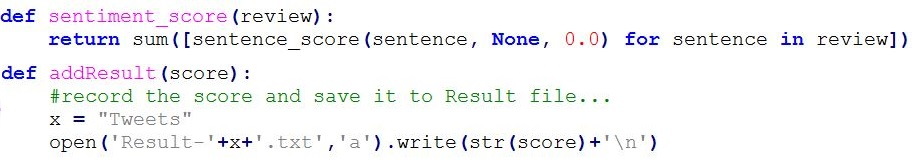
\includegraphics[height=2.5cm]{images/AddResult.jpg}
\end{center}
\hspace*{\parindent}\textbf{\large \#7 : Dictionary updating }
\begin{center}
	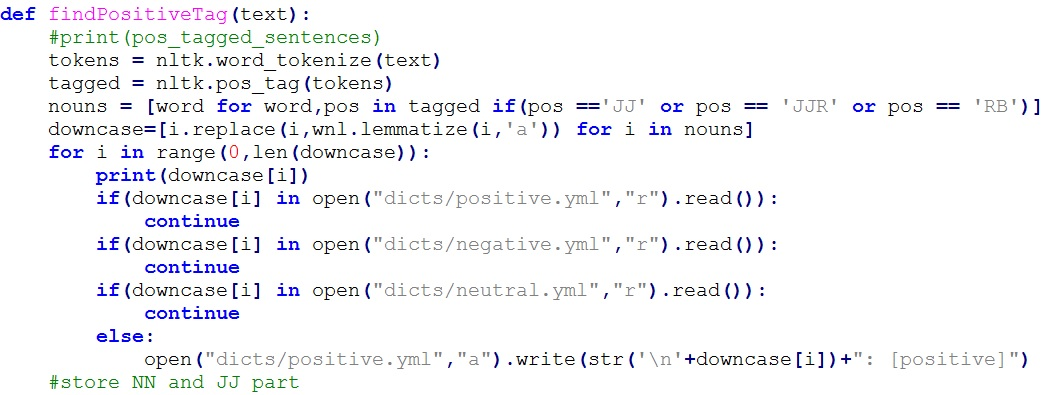
\includegraphics[height=6cm]{images/DicUpdate.jpg}
\end{center}
\end{appendices}
\newpage
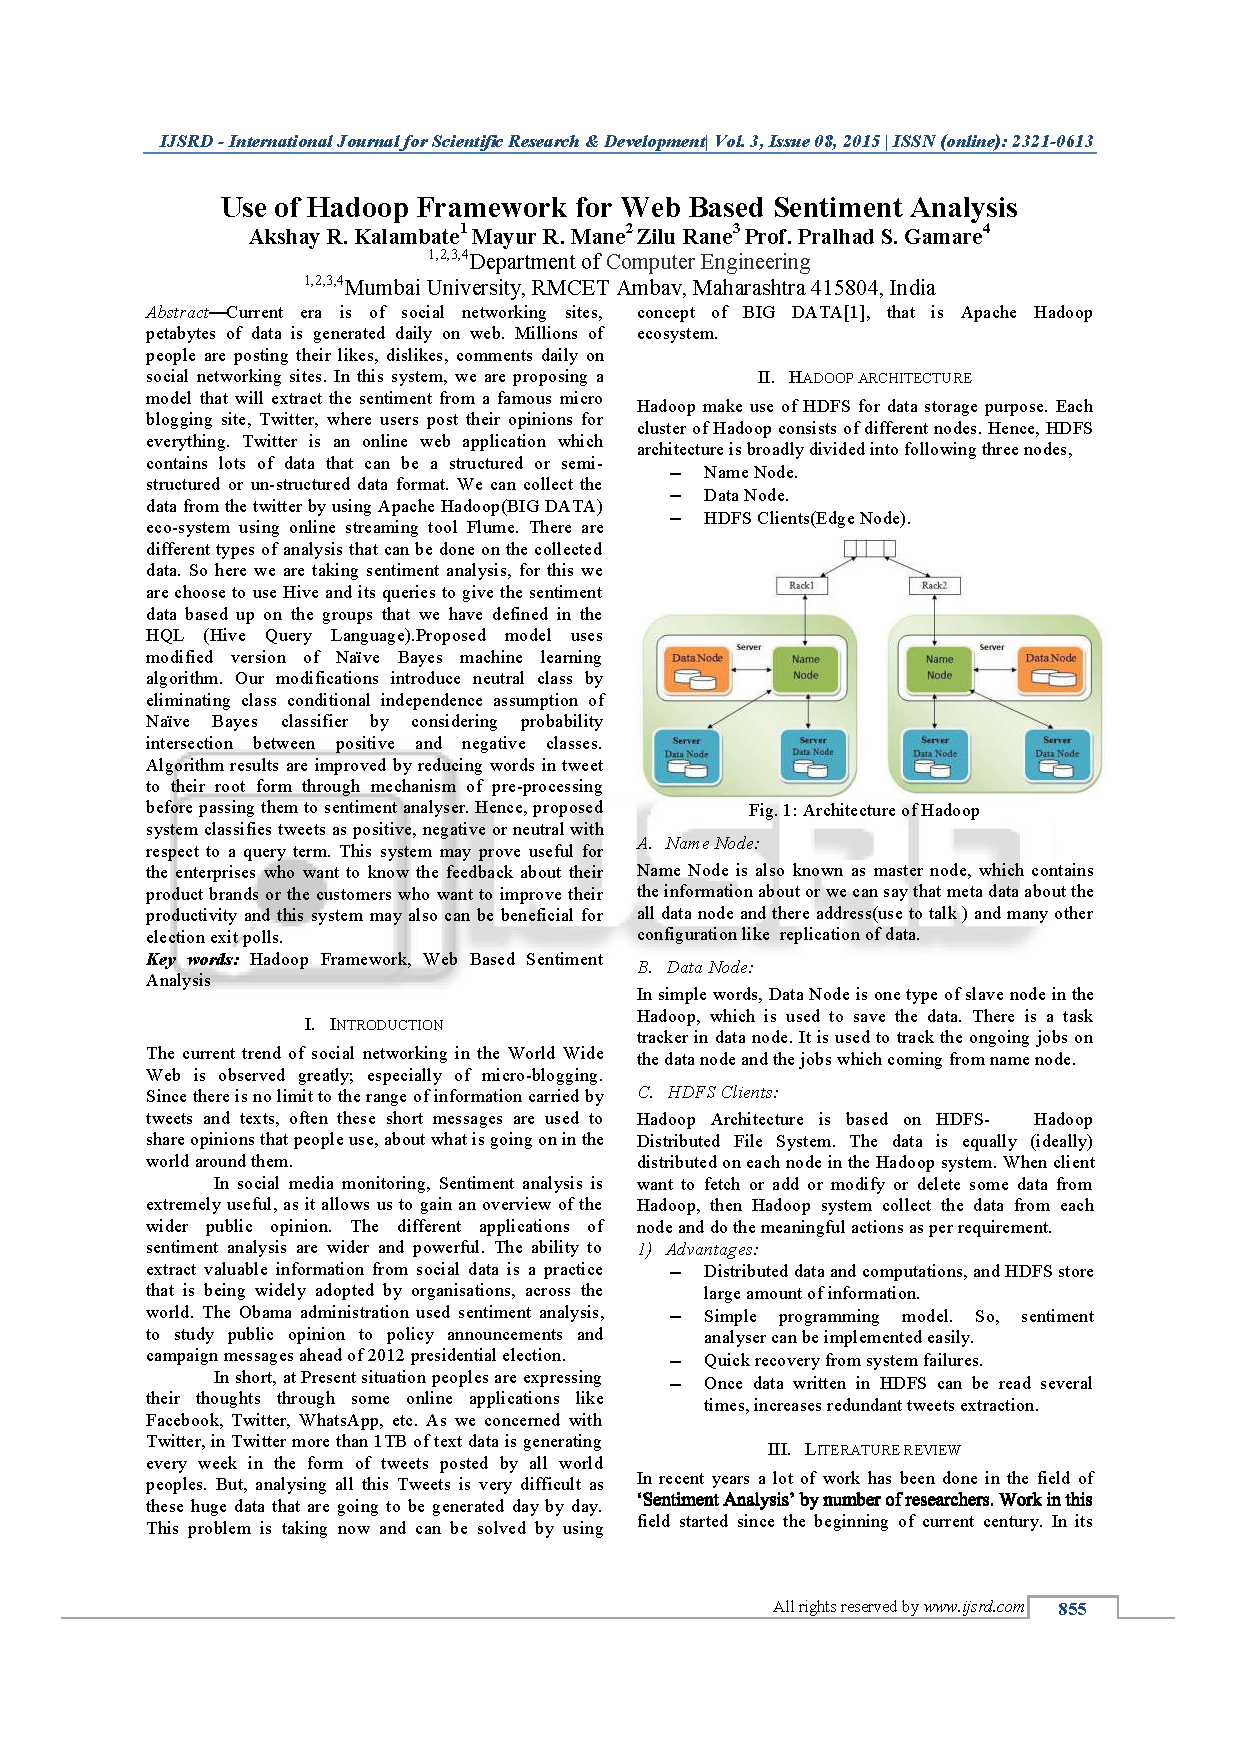
\includepdf[pages={1-3}]{IJSRDV3I80379p.pdf}

\includepdf[pages={1}]{acceptanceletter.pdf}
\addcontentsline{toc}{chapter}{Publications}
\newpage

\begin{center}
{\huge \bf {ACKNOWLEDGEMENT}}
\end{center}
\vspace{10mm}
\hspace*{\parindent}We would like to express our sincere gratitude towards our guide, Prof. P. S. Gamare, for the help, guidance and encouragement, he provided during the B. E. Project. This work would have not been possible without his valuable time, patience and motivation. We would like to thank him for making our stint thoroughly pleasant and enriching. It was great learning and an honor being his students. We are deeply indebted to Prof. L. S. Naik (Head of Department) and Prof. P. S. Gamare (Project Coordinator) and the entire team in the Computer Department. They supported us with scientific guidance, advice and encouragement, they were always helpful and enthusiastic and this inspired us in our work. We take the privilege to express our sincere thanks to Dr. M. M. Bhagwat, our Principal for providing the encouragement and much support throughout our work.
\vfill
\begin{flushright}
\begin{tabular}{p{60mm}}
\vspace{5mm}
{ {Mr. Rane Zilu Ramkrishna}}\\
\vspace{5mm}
{ {Mr. Mane Mayur Ravindra}}\\
\vspace{5mm}
{ {Mr. Kalambate Akshay Rajendra}}
\end{tabular}
\end{flushright}
\vfill
\newpage
\begin{center}
{\huge \bf {AUTHORS}}\\
\end{center}
\vspace{10mm}
\def\baselinestretch{1}
\begin{framed}
\centering
\fbox{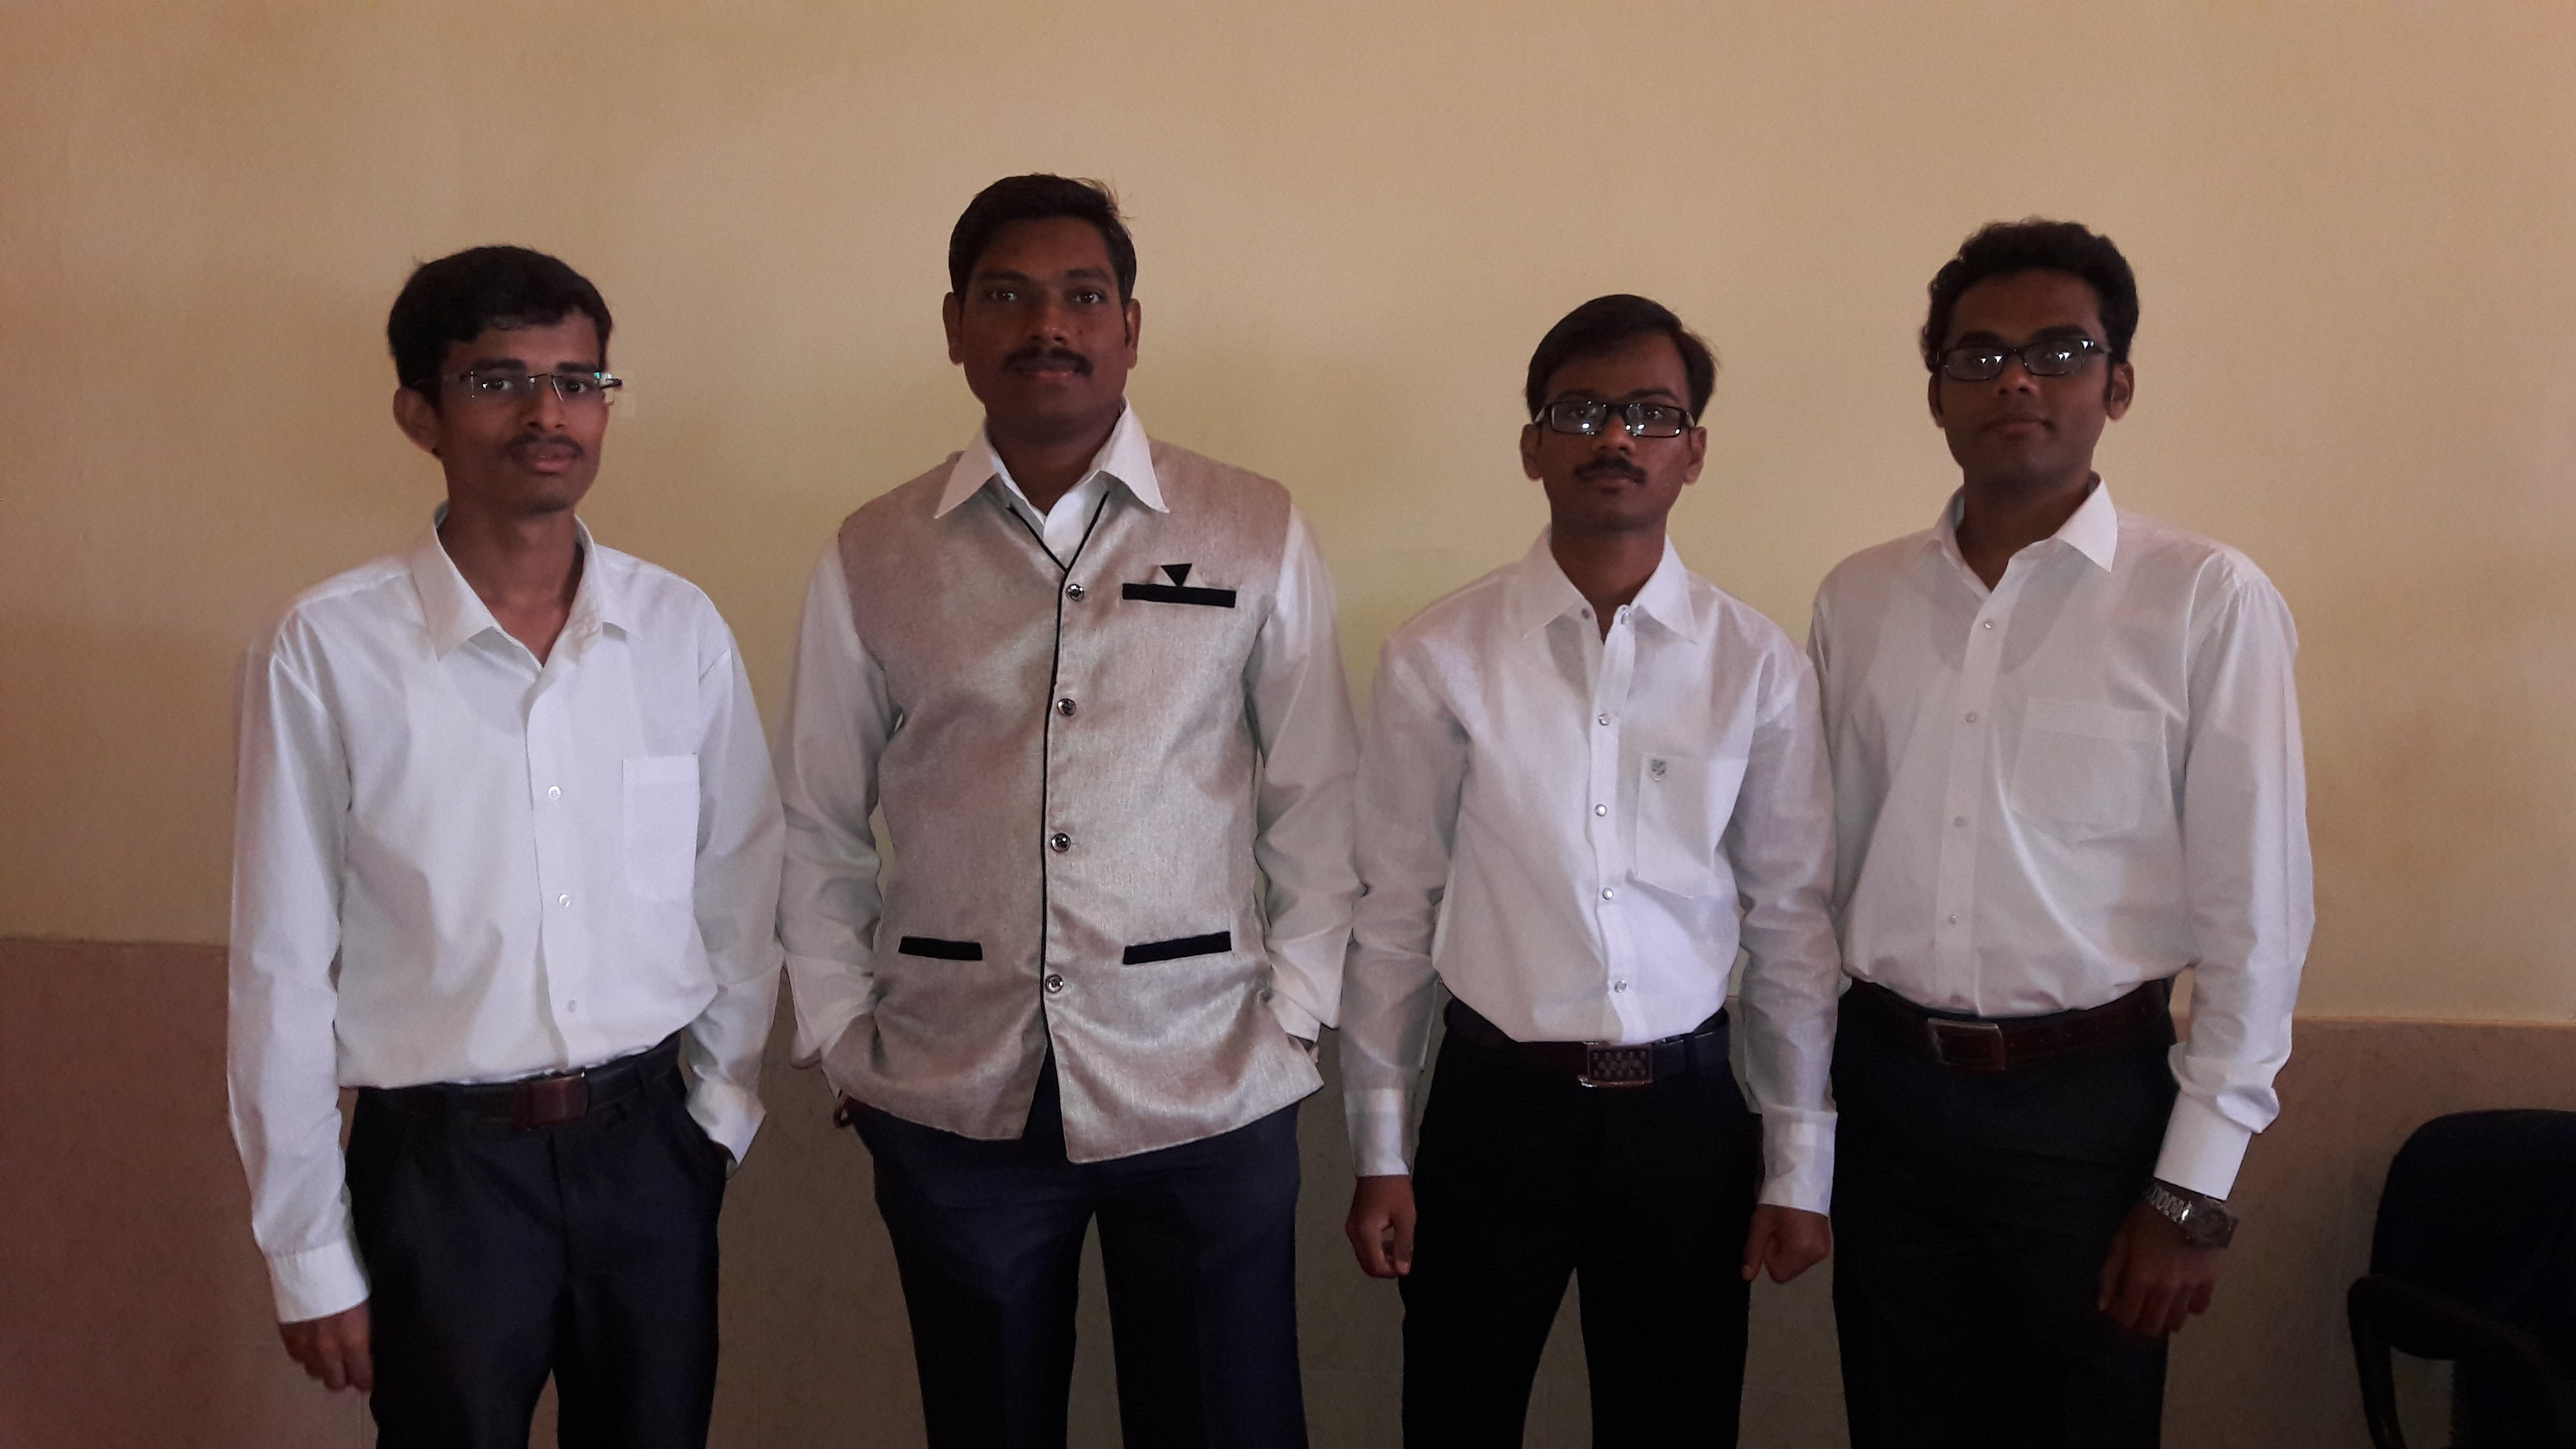
\includegraphics[width=15cm]{images/team.jpg}}
\captionof*{figure}{Authors from left Mr. Zilu Rane, Prof. Pralhad Gamare, Mr. Akshay Kalambate and\\ Mr. Mayur Mane}
\end{framed}
\bf \large
\hspace{20mm}
\begin{enumerate}
   \item Mr. Zilu Ramkrishna Rane {(\underline{zilurrane@gmail.com})}
	\item Mr. Mayur Ravindra Mane {(\underline{mayoorm909@gmail.com})}
	\item Mr. Akshay Rajendra Kalambate {(\underline{akshaykalambate15@gmail.com})}
	\item Prof. Pralhad S. Gamare {(\underline{pralhad.gamare81@gmail.com})}
\end{enumerate}

\end{document}
%This template is designed by Zilu Rane and whole team of compilers
%So if your are using template so dont forget us
